\documentclass[
  final,
  babelLanguage=hungarian,
  desktopVersion,
  %showtrims,
  %overleaf,
]{anecdote}

%\graphicspath{{./assets/photos/300dpi/}}
\graphicspath{{./assets/photos/92dpi/}}

% Page size: 135 x 120 mm
% Body text: 11 / 14 pt

\usepackage{local}

%% Details of the book
%% ===================

\title{Szótlanul Kérdem}
\subtitle{bevezető a buddhista meditációba és szemléletbe}
\author{Gambhíró Bhikkhu}
\publisher{Kiadó}% TODO
\date{2019-10-04}
\editionInfo{\textit{Első kiadás}, 2019}% TODO update edition info
\ISBN{000-000-0000-00-0}% TODO update ISBN

% === Metadata ===

\hypersetup{
  pdftitle={\thetitle},
  pdfauthor={\theauthor},
  pdfcopyright={Copyright (C) 2019, \thePublisher},
  pdfsubject={},% TODO subject
  pdfkeywords={},% TODO keywords
  pdflicenseurl={https://creativecommons.org/licenses/by-nc-nd/4.0/},
  pdfcontacturl={},
  pdflang={hu},
}

%% === Load further packages ===

%% === Hyphenation exceptions and corrections ===

\hyphenation{London}

\begin{document}

\frontmatter

%\ifdesktopversion
%\desktopCover{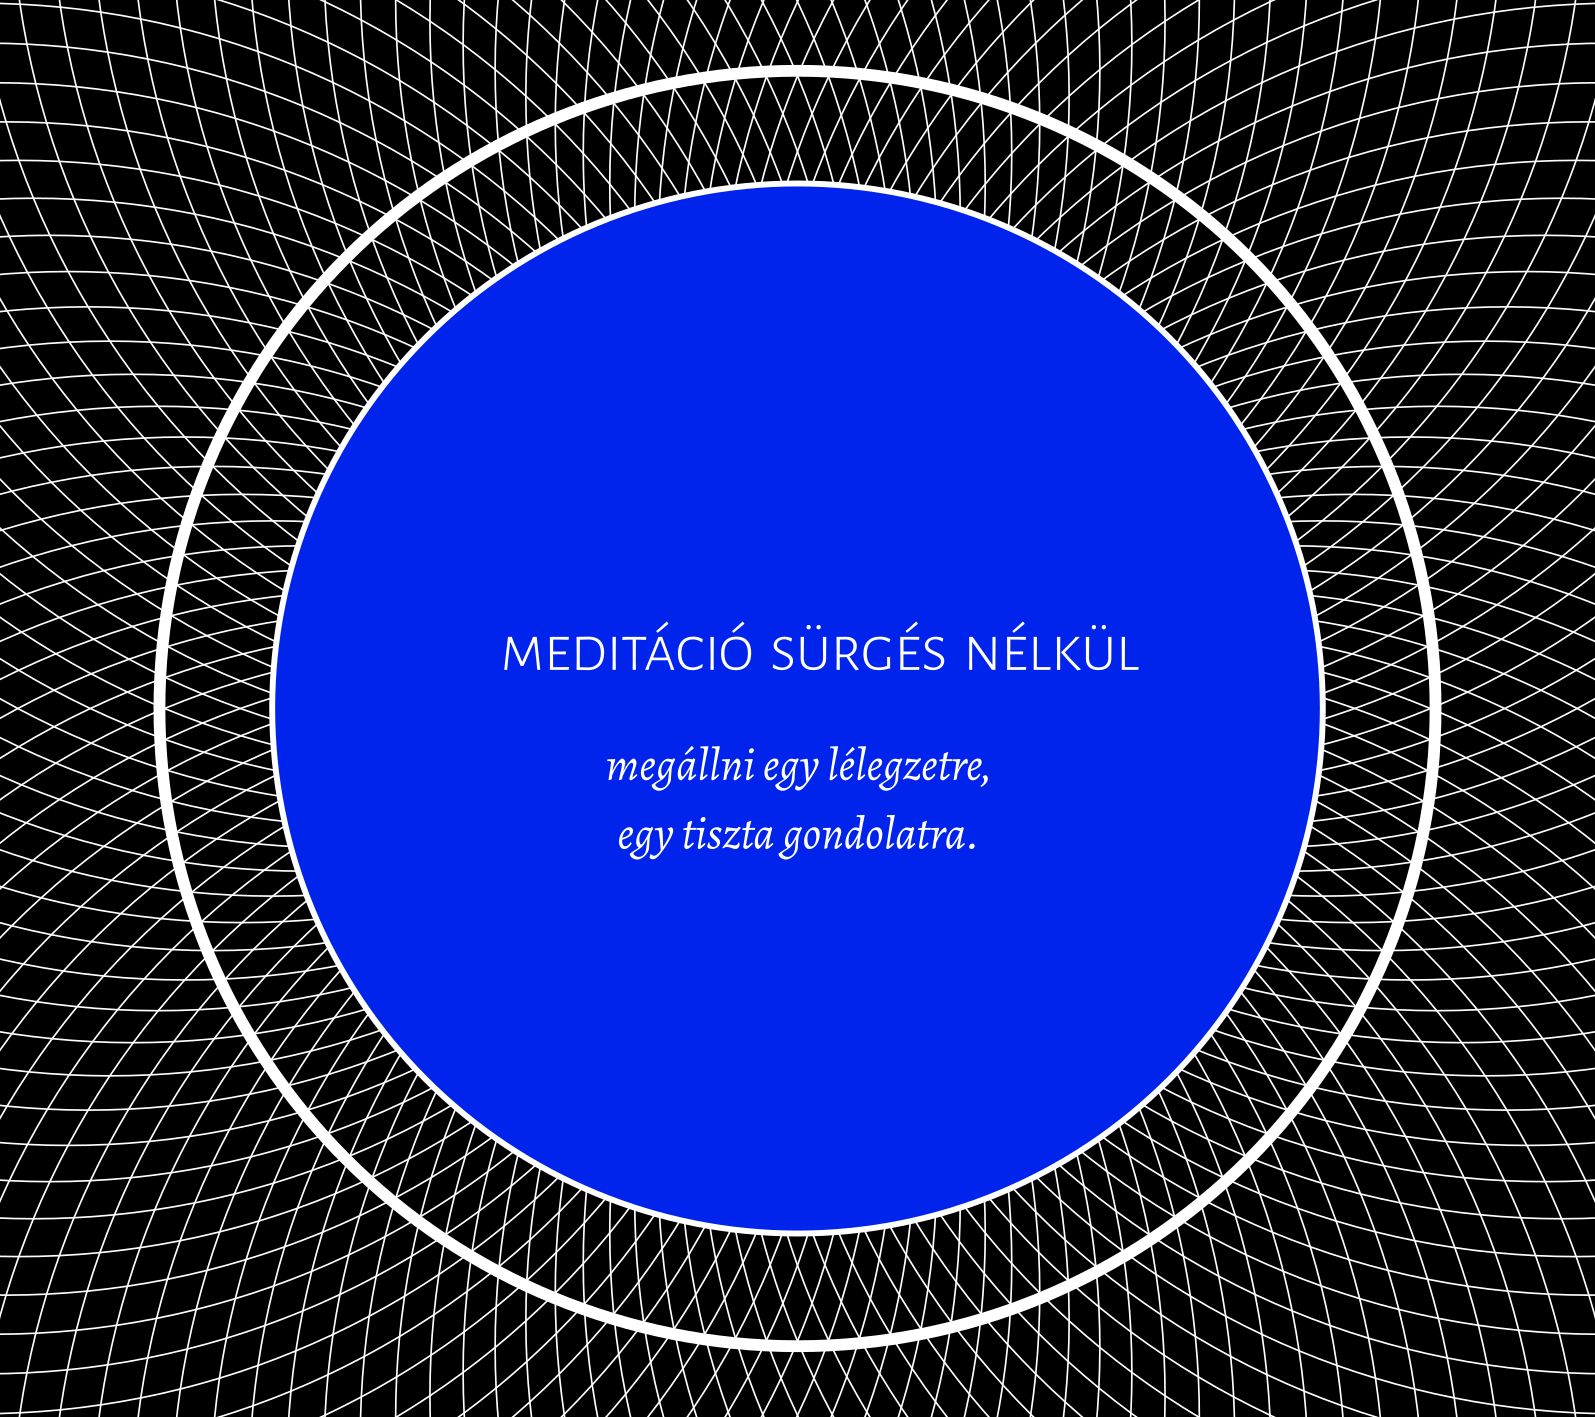
\includegraphics[height=\paperheight]{./desktop-cover-hu.png}}
%\fi

\cleartorecto
\thispagestyle{empty}
\vspace*{5em}

{\centering

{\Large\alegreyaSansScLightFont\selectfont\MakeLowercase{\textls*{\thetitle}}}\\[5pt]
{\chapterTitleFont\selectfont\itshape \thesubtitle}

\vfill

{\chapterTitleFont \theauthor}

\vspace*{2em}

}



%\cleartoverso
\thispagestyle{empty}

{\copyrightsize
\centering
\setlength{\parindent}{0pt}%
\setlength{\parskip}{0.8\baselineskip}%

\thetitle\\
by \theauthor

% Published by \thePublisher
% 
% ISBN \theISBN
% 
% Copyright \copyright\ \thePublisher\ 2019
% 
% Cover Photograph: The Person

\vfill

This work is licensed under a Creative Commons\\
Attribution-NonCommercial-NoDerivatives 4.0 International~License.

Produced with the \LaTeX\ typesetting system, set in Crimson Roman and Alegreya Sans.

% \theEditionInfo

}

%
%\cleartorecto
\thispagestyle{empty}

\mbox{}\vfill

\noindent
{\itshape
  \ldots\ Ezért a bölcs\\
  sürgés nélkül működik,\\
  szó nélkül tanít,\\
  nézi az áramlást és hagyja, nem erőlködik\ldots
}

\bigskip

\noindent
{\smaller Tao Te King, ford. Weöres Sándor}

\vfill\mbox{}


\cleartorecto
\tableofcontents*

%\input{./manuscript/tex/foreword.tex}

%\input{./manuscript/tex/preface.tex}

% Page 1 is the first page of the first chapter.
\mainmatter

\chapter{Légzés}

\keywords{\emph{ānāpānasati} módszer és testtartás röviden}

\noindent A lélegzet érzéseit figyeljük a testben, ez az éber figyelem
az elmét egy stabil tárgy köré gyűjti össze. A test érzései jól
észrevehetőek miközben be- és ki lélegzünk. Ez a módszer
\emph{ānāpānasati} néven ismert, vagyis éberség a lélegzetre.

Miért annyira fárasztó a sok gondolkodás? Az elme egyik gondolattól a
másikig ugrál, de nem tudjuk hova megyünk és így sosem érkezünk meg. A
nyugtalan vágy kimerítő. Az érzéki visszafogottság összegyűjti az
energiát és irányítja azt, nem engedi szétfolyni minden irányba. A
figyelmet egy semleges, egyenletes érzésre irányítjuk, ami lelassítja a
gondolkodó elmét.

Ülhetsz a padlón, a szőnyeget és egy párnát használva, vagy egy széken
is. A padlón ülve, találj olyan helyzetet, ami nem erőlteti túl az
inakat vagy térdeket.

Széken ülve, húzódj előre az ülésen, hogy a hátad ne támaszd a
háttámlának. A támasz befolyásolja a gerinc alakját, és a légzés
ritmusát.

Tartsd a fejet egyensúlyban úgy, hogy a súlya ne húzzon előre. Mivel
gyakran széken ülünk, szokásunk a fejet előre tartani, ami a hátizmokban
hoz létre feszültséget. A fejet egy kicsit hátrahúzva érezzük, hogy
ellazulnak a hátizmok. Jó, ha az áll kissé behúzódik, de nem kell
erőltetni.

Ülj egyenesen, kiegyensúlyozott testtartásban, a vállakat ellazítva. Jó
tartással a légzés könnyű és egyenletes.

\clearpage
\null\thispagestyle{empty}%
\photoFullBleed{sitting.jpg}%
\illustration{Ülő Meditáció Tesstartás}%
\label{illus-sitting-meditation}%
\clearpage

A test csontjai úgy ülnek egymáson mint egy kövekből rakott torony. A
csípő-csont a párnán nyugszik, a gerinc a csípőn, a gerinc-korongok
egymásra rakva, a tetején a koponya, az egész torony középvonala
óvatosan egyensúlyban tartva.

Ha óvatosan ki van egyensúlyozva, és a súlypont középen van, nem
szükséges az izmok erejével húzni-vonni a testet, hogy megtartsuk. A
gravitáció elég ahhoz, egyenesben tartsa.

Belégzéskor, a hideg levegőt először az orrhegynél érezzük. Hagyd, hogy
a hasizmok irányítsák a levegővételt, ahelyett, hogy a mellkast tágítva
növelnéd a térfogatot. A levegő áthalad a tüdőn, és a has kitágul; ez a
légzési módszer csökkenti a szívritmust és feszültséget. Ellazítjuk az
izmokat, és a levegő az orron át távozik. Nem kell ezt precízen
irányítanunk, elegendő finoman utalni erre a ritmusra. A test magától is
tudja hogyan kell lélegezni, visszalépünk és figyelünk, mintha
hullámokat néznénk ahogy besodródnak a partra, majd visszahúzódnak.

Nem kell megmondanunk magunknak mit gondoljunk és mit érezzünk. Ha
tiszta gondolatokat akarunk, legjobb először csendben lenni és figyelni.
Csendben ülünk és pihenünk egy kis ideig. Mikor elhallgatunk, vagy
tiszta gondolatok jönnek maguktól, vagy az elme elégedett lesz a
csenddel együtt maradni.

Visszafogottság és irányított figyelem szükséges a tiszta, tudatos
gondolathoz -- és ez békés örömet hoz magával. Az elme elégedett és
boldog, nem érzi szükségét a sok belső párbeszédnek. Leülni és
lélegezni, a csendet hallgatni magában is egy hibátlan öröm.

Megalapozzuk a tiszta szándékot, hogy a meditáció tárgyával maradunk és
más ügyeket későbbre hagyunk. Segít a nyitott hozzáállás, erővel
kényszeríteni magunkat nem elég érzékeny, hogy lássuk mi történik.
Akaraterővel irányítva a meditáció merevvé válik, és az elme
akadályozott lesz. Mintha gyorsan akarnánk menetelni merev lábakkal, és
felbukunk a kavicsokban.

A tiszta elme és jó elhatározás érzése nyugodt és hűvös, nyitott a
változásra. Az erőltetett küszködés érzése elfoglalt és forró, szűk a
látótere.

\keywords{hozzáállás a módszerhez, az elme nem egy kávégép}

Tanulunk új tényeket az elméről azzal, hogy a légzést figyeljük?
Emlékszem, amikor nekiültem és azzal küszködtem, hogyan kellene
\emph{helyesen} meditálnom. Folyton ezen gondolkodtam és a légzésemen
változtatgattam hogy javítsak a meditációmon, arra számítva, hogy egy
nap majd valahogy megnyomom a helyes gombokat, és a helyes módon
lélegezve elkezdek új információkat, új tényeket megismerni az elméről.
Elég fájdalmas folyamat volt, és teljesen eredménytelen.

A tudást keresve analizálunk, és közben lemaradunk arról, ami történik.
Gondolj egy beszélgetésre, mikor a másik folyton azt kérdezi,
``Miért?'', minden mondatod után -- a beszélgetés sehova nem jut
hallgató figyelem nélkül. Ezt tesszük magunkkal miközben túlagyaljuk a
meditációt; nem is csoda, hogy fel akarunk ugrani az ülőpárnáról és
megmondani a kommentáló elménknek, hogy hagyja abba és figyeljen
csendben.

A tanítóink utasításai a figyelmünk olyan irányítására vezetnek rá,
amivel a magunk számára felfedezhetjük a megértést.

Tanulunk az olvasott vagy hallott utasításokból, de amikor
\emph{pontosan, precízen, helyesen} próbáljuk követni ezeket, olyan,
mintha a kézikönyvet olvasnánk egy kávégép működtetéséhez: `Ha megnyomom
ezt a gombot, mindig ilyen kávét kellene készítsen'.

Ezt a hozzáállást az motiválja, hogy irányítani és manipulálni akarjuk
az élményeinket, de frusztrációt tapasztalunk, mert természetük szerint
nincsenek az irányításunk alatt. Már előre eldöntöttük mi lesz. Azt
akarjuk látni, amit \emph{gondolunk}, hogy történnie kellene, és nem
látjuk ami \emph{valóban} történik, ezért azt gondoljuk a gép nem
működik, vagy mi használjuk rosszul.

Emlékeztethetjük magunkat, hogy lehetséges, hogy nem tudunk mindent. Nem
tudjuk mi fog történni. Lazíts a tartáson, gyakorold a hozzáállást ami
megáll és figyel.

\keywords{BUD-DHÓ mantra, erőfeszítés és frusztráció}

Kezdhetjük a BUD-DHÓ mantra gyakorlásával, magunkban ismételve a be- és
kilégzéskor. `Buddhó' azt jelenti, `aki éber, aki megismer'. Segít
megállni és figyelni.

Ez felébreszti az elmét, hogy ismerje önmagát ahogy épp most van. Az
ébredés mindig helyes -- nem tudod elrontani. Az elme felismeri a saját
változó természetét, a gondolatok szavai szükségtelenné válnak, és a
figyelem megtalálja a szótlan kérdést ami a jelennel együtt marad.

Az erőfeszítés szükséges, és az elme akadályai miatt nehéz feladatot tud
jelenteni, hogy ne adjuk fel a gyakorlást. Újra és újra, visszatérünk az
elméhez ami éber a jelen tapasztalatra és ez irányítja az erőfeszítést,
az akaratos törtetés helyett egy cél felé.

A frusztráció és csalódás hasznos jelzések arra, hogy figyeljünk -- a
legjobb, amikor olyan dolgot kell megtanulnunk, amire nem számítottunk,
hogy erre jobban kell figyelnünk.

Nem szükséges sokat olvasnunk, vagy sok mindenre emlékeznünk. Kevés
információra van szükségünk, de kifejleszteni a jártasságot ezekben sok
gyakorlást igényel. Gyakori hibánk, hogy nem állunk meg, hogy velük
maradjunk, és kicsomagoljuk a jelentésüket arra, hogy felismerjük a
pillanatnyi helyzetünket, \emph{mit tegyünk} és \emph{milyen módon
tegyük azt}.

Egy sor tény, ha nem építjük be őket, nem érnek le elég mélyre, hogy a
szív és elme tapasztalatainak gyökereit kezeljék, és nincsenek ránk
hatással. A lélegzet figyelése megállít minket, és megnyílik a
figyelmünk, ami képes ezt elérni. Az észrevételek és megismerés
fokozatos lehet, mint amikor közel kell hajolnunk valamihez, hogy
lássunk egy lényeges részletet, de minden lépés, amivel összekötjük a
saját tapasztaltunkat a tanítás szavaival, érdekes és tovább vezet.

A Buddhának egy egyszerű üzenete van számunkra: ébredj fel, ne
ragaszkodj, nem kell szenvedned. Ezt csomagoljuk ki, egyre szélesebbre
tárva.

\section{Vezetett meditáció}

\keywords{\emph{ānāpānasati} módszer, ülő meditáció, ülő tesstartás}

\enlargethispage*{\baselineskip}

Igazítsd ahogy ülsz, és találj egy kiegyensúlyozott testtartást: a
tartásod egyenes legyen, stabil de nem feszes helyzetben, a fej legyen
egyensúlyban és ne dőljön előre. A tartásod engedje a nyitott, könnyű
légzést.

Határozd el, hogy erre az időre félreteszed a mindennapi
tevékenységeket. Válaszolhatsz a megszakító gondolatokra, `Ez nem a
megfelelő idő, később vissza fogok erre térni amikor az idő alkalmas
rá.' Hosszabb, mint az, hogy `Csend legyen!', de barátságosabb magunkkal
szemben. Ez megalapoz egy tiszta szándékot az elmében, mint elpakolni az
asztalról mielőtt dolgozni kezdünk.

Vegyél egy mély lélegzetet, és figyeld, hogy érzel-e feszültséget,
valamit ami akadályozza vagy korlátozza a légzést. Ha úgy érzed, a
légzés könnyű és nyitott, a testtartásod megfelelő. Nem kell különleges
módon ülnöd.

Figyelj a légzés testi érzéseire. Engedd, hogy a test szabályozza a
légzést, mi csak figyeljük és hagyjuk ellazulni, arra figyelve ami éppen
történik.

A jó testtartás és a nyugodt, könnyű légzés egy csendes és örömteli
érzés, mint leülni a parkban egy padra egy séta után. Semmi különös
dolgunk nincs, és ez az egyszerű, csendes ülés magában is öröm.

A légzést nem irányítjuk olyan precízen, mint egy pránajáma vagy jóga
gyakorlat közben, viszont érdemes figyelni milyen testi ritmus irányítja
a légzésünket.

Ha a légzést a mellkas tágulása és összehúzódása irányítja, mintha nagy
erőfeszítésre készülnénk, ez mozgásra ösztönöz és aktívabban gondolkodó
elmét produkál. Megnyugtató hatással van, ha inkább a has feletti
rekeszizom irányítja a légzést. Ha egyszer megvan a ritmusa, hagyd a
testet, hogy magától folytassa.

\enlargethispage*{\baselineskip}

Belégzéskor, a levegőt először az orrhegynél érezzük. A hideg levegő
lefelé áramlik a légcsövön. A has kifelé mozdul, engedve a rekeszizom
tágulásának. A mellkas emelkedik, miközben a tüdőt kitölti a levegő, de
nem kell nagyra tágítani a mellkast. Nyugodtan ülünk, érezhetjük a
szívverés halk ritmusát.

\clearpage
\null\thispagestyle{empty}%
\photoFullBleed{breathing.jpg}%
\illustration{Légzés Technika}%
\label{illus-breathing}%
\clearpage

Kilégzéskor az izmok ellazulnak, a meleg levegő felfelé áramlik a
légcsövön, és az orron át távozik.

Nem szükséges ezeket a lépéseket gondolatban kifejezni, lazíts és
figyeld, ahogy az érzések megjelennek a testben. Eltart pár percig, amíg
a test megállapodik. A szívverés lecsillapodik, és a légzés egyenletes
és könnyű lesz.

Hagyd, hogy a test maga szabályozza a légzést. Amikor egy véleménnyel
állunk hozzá, hogy a légzésünk rövid legyen, vagy hosszú, az merevvé és
erőltetetté válik. Fel akarjuk fedezni a tapasztalatainkat, nem
megszabni, mik legyenek azok.

A test jobban tudja hogyan kell lélegezni, mint mi. Egyenletesen fog
lélegezni, ha hagyjuk. Lépj egyet vissza és fordítsd meg a figyelmet,
hallgatózz ahelyett, hogy utasítasz. Belégzés, kilégzés, mit érzel a
testben?

Nincs semmilyen meghatározott érzés, amit tapasztalnod kell. A szándék
az, hogy adj időt, és engedj teret annak, hogy a tapasztalataiddal
maradj.

Egyensúlyban önmaga középpontjában, ismerni a jelen pillanat
egyszerűségét. Ha úgy érzed, hogy valamit teljesítened vagy javítanod
kell, ez mindig egy hozzáadott dolog, valami amit mi hozunk létre. Mi
hozzuk létre az elvárást, hogy változtatnunk kell, ki kell valamit
javítanunk, irányítanunk kell. Ez mindig az időhöz kötött, valamit
elvárunk, hogy történni fog.

\enlargethispage*{2\baselineskip}

A jelen pillanatban minden mozgásban, változásban van. Az azonnal, a
jelenben megtapasztalható élményben nincsenek célok. Nincsenek a jövőben
megjelenő eredmények, csak \emph{ez, itt} van. Azok az elvárások, amiket
magunk számára produkálunk, szétfoszlanak, amikor visszafordítjuk a
figyelmet, és a jelent figyeljük.

Visszatérünk a figyelemhez, ami az itt és most tapasztalathoz kötődik.
Az érzékeken keresztül felismeri a világot. Ebben a figyelemben a
kétségek, kérdések, emlékek, nem súlyosak. Nincs olyan súlyuk, nincs
olyan sürgető jelentőségük, ami minket kimozdítana az egyensúlyból. Ez
az éber figyelem egy biztonságos hellyé válik, ahol maradni tudunk.

Lehet, hogy sok kusza gondolat jár az elmében. Határozd el mit fogsz
gondolni, ahelyett, hogy hagynád az elmét körbe-körbe járni. Például
használd a BUD-DHÓ mantrát. A belégzéskor, gondold BUD-, kilégzéskor,
-DHÓ. Ha a gondolkodás nem csillapodik le magától, ez oldalkorlátot és
fekvő-rendőrt rak le, hogy az úton maradjunk és lassítsunk.

\keywords{aktív és nyugodt elme, kavargó érzelmek, a jelen egyszerűsége}

Belélegzünk, maradunk a jelen egyszerű tapasztalatával: ennyi elég.

Kényszereket érzünk, vágyakat és aggodalmakat, úgy érezzük, `erre
szükségem van', `én ilyen vagyok', `olyannak kellene lennem'. Ezeket
éberen szemlélni tudjuk, nem kell belekeverednünk a történetbe. A
légzéssel maradunk, és figyelmünket a tapasztalat felé fordítjuk, ami
éppen történik.

A testi éberség egy szilárd alap, megnyugtató és átrendezi mi az
értékes. Ha a tapasztalatod békés, boldog és elégedett, maradj vele.
Nincs abban semmi rossz. Ez egy olyan boldogság, ami nem kötődik a
ragaszkodáshoz, nem függ attól, hogy megszerezzünk vagy elérjünk
valamit. Ez a boldogság az érzékek elvonultságából ered, visszatérve az
egyszerűséghez, megismeri és együtt marad a jelennel. Az elme éber,
nyugodt és elégedett.

A meditáció a kavargó érzelmeket is a felszínre hozza, és ez jól van
így. Azt látjuk, amit eddig nem engedtünk magunknak, hogy lássunk. Nincs
szükség arra, hogy válaszokat és megoldásokat keressünk meditáció
közben. Az érzelmeket nem a személyes történetünk szintjén vizsgáljuk,
hanem alapvetőbb szinten, mint az elme és szív állapotait.

Magunkat látjuk bennük, sajátunknak tekintjük ezeket, és ebből hozunk
létre egy személyt, akinek a történetét irányítani akarjuk. A jelen
tapasztalatban viszont sem az érzés, sem az elmeállapot nem jelenti be
magáról, hogy kinek a nevéhez tartozik. A szenvedés és nehézség ebből a
ragaszkodásból és zavaros nézetből ered. Nyitni kell az elmét a
változásra, és elengedni a ragaszkodást.

\keywords{jótékony gondolatok, túl komoly hozzáállás}

Az erény, a nagylelkűség ellazítja az elmét, a moralitás pedig stabil
alapot ad. Gondolhatunk jó tettekre, amit adtunk és kaptunk,
emlékezhetünk azokra, akikre jó példaként tisztelettel nézünk fel.

Ha azt veszed észre, hogy feszült vagy, szigorú és cinikus a hangulatod,
igazíts a testtartáson, hogy kicsit lazább legyen.

Olyan komolyak tudunk lenni abban, hogy egy párnán ülünk, kész vicc ránk
nézni. Csendben dörzsöld meg a füleid, vagy masszírozd meg az arc
izmokat az ujjaiddal, ez serkenti a vérkeringést. Emlékezz a
nagylelkűségre. A kolostorban gyakran a világi barátaink azok, akik
eljönnek főzni és felajánlani a napi ebédet a közösség számára. Nagy a
sürgés-forgás amíg a konyhában vannak, és amikor végeztek,
megkönnyebbültek, lazítanak és mosolyognak.

\enlargethispage*{\baselineskip}

Felidézni jó tetteinket, egyszerű kis dolgok esetében is, ellazítja az
eredményekre szomjas elmét. Képzeld el mi történne, ha valaki
százszorosan megadná neked az eredményt amit akarsz, mintha megnyernél
egy megvilágosodási lottót. Akkor hogy meditálnál? Valószínűleg közel
úgy mint most, csak lazábban.

A nagylelkűség enged felismerni, hogy van elég terünk, nem kell
erőlködnünk, hogy mások elé jussunk. Van jóság a világban és
felhagyhatunk a nagy sietséggel. Örömteli érzés felidézni a családunk,
rokonaink és barátaink nagylelkűségét is, de még amikor egy ismeretlen
embert látunk segíteni egy másik ismeretlennek, az is előcsal egy
mosolyt.

\keywords{kétség a meditációban, érzékek befelé fordulnak}

`Hogy tudom megcsinálni?' Közelítsd meg másként, és inkább azt kérdezd,
`Tudok rá figyelni?'

A légzés érzete megállít. Visszakerülünk az elejére, ahol nem tudjuk mi
lesz. Egy üres és tágas helyre kerülünk így, ahol magunk vagyunk és van
időnk ott megállni.

A légzésre figyelve az érzékek befelé fordulnak. A szem látja a
színeket, de a látás befelé irányul, nem akar kívül színeket és formákat
keresni. A fül hallja a hangokat, de a hallás befelé fordul és nem
keres. A test érzi a hideget, meleget, a ruhák felületét és a csontok
merev súlyát. A légzés közben figyeljük ezt és hagyjuk a testet
lenyugodni, hagyjuk az elmét befelé fordulva elcsendesedni.

\enlargethispage*{2\baselineskip}

\keywords{hűvös víz szétárad a tóban, a tapasztalat tartalmazza a világot}

Az érzéki visszafogottság összegyűjti az energiánkat és nem engedi
szétfolyni minden irányba. Mint egy tó, aminek nincsenek ki- és bevezető
folyásai, határait körben a völgy szabja meg. Csupán egyetlen, a földből
feltörő forrásból kap hűvös, friss vizet. Amikor eső esik, némi víz kis
erekben a tóba fog folyni, de mivel nincs kifolyása, mind a tóban fog
megállni és a völgy határt szab neki. A tó vize nyugodt marad, és a
forrás hűvös vize az egész tóban szét fog áradni, áthatja annak minden
részét.\footnote{\href{https://a-buddha-ujja.hu/dn-2/hu/csimma-vilmos}{DN
  2}, A szerzetesi élet gyümölcsei}

Az érzés és tudat a testtől függ, nem tudunk hozzátenni vagy elvenni
belőle. A tapasztalat minden légzésben teljes, a testtel kezdődik és
azzal lesz vége. Ez a világ, ami érzésekből áll, ebben teljes -- minden
ami vagyunk, vagy amivé valaha válhatunk, ezen belül van.

\keywords{a tudatosság megállítja a kényszert}

Amikor szenvedünk, tudjuk, hogy van itt valami, amit nem értünk. Nem
értjük, hogy egy dolog hogyan jött létre a másikból, hogy egy dolog az
irányításunk alatt van, a másik pedig nincs.

Amikor nem látjuk, ugyanazt a mintát ismételjük, mint egy programot, és
ugyanazt a szenvedést újra és újra létrehozzuk. Panaszkodunk, hogy
`Miért van ez mindig így?' Ugyanazt a dolgot tesszük újra és újra, és
nem vesszük észre.

Közelebbről megvizsgálva felismerjük, hogy az egyik dolog a másiktól
függ. Akkor látjuk a lehetőséget, hogy szabadon abbahagyhatjuk. Így
visszatérünk a csendes elégedettséghez.

\keywords{nyugtalanság, önkritizálás, jó szándékkal kezdeni, rugalmas hozzáállás}

Amikor már egy ideje meditálva ülünk, gyakran elkezdjük bonyolítani a
dolgot. Honnan jön ez a nyugtalanság, hogy nem tudunk egy egyszerű
dologgal együtt maradni? Figyeld meg, ahogy az egyszerűbe vetett hit
megváltozik. Elkezdünk valamilyen szempontról vagy kérdésről
gondolkodni, és a kétség és önkritizálás megállít mindent.

\enlargethispage*{\baselineskip}

Nem komikus ez? Olyan elkötelezetten tudjuk kritizálni magunkat, mintha
egy túlemelkedett élmény lenne az, hogy fájdalmat okozunk magunknak. De
úgy érezzük, erőlködnünk kell \emph{valamin}, meg kell törjük az egónkat
és el kell engedjünk mindent! Talán csak ezt az egy módszert ismerjük,
nem is tudjuk milyen lehet nem ilyennek lenni.

Az elején megvan az önmagunkkal szembeni jó szándékunk és rugalmas
hozzáállásunk, de a végén csak keménység és bírálat marad. A fiatal fa
friss és rugalmas, könnyen hajlik ahogy nő, de az öreg fa kemény és
száraz amikor elpusztul.

Térj vissza az elejére, ahol megvan a kezdővel szembeni türelmed és
kedvességed. Az elején még nem vártad el magadtól, hogy tudnod kell, és
a hallgató figyelemre hagytad, hogy lásd, mi történik. Nem tudjuk, mi
van itt, amíg meg nem nézzük, hogy lássunk. Ez a látás és figyelem a
friss megismerés. Engedd magadnak, hogy mindig az elején legyél.

\chapter{Megértés}

\keywords{tények és tapasztalat, kétség, tények halmozása}

\noindent Részekre osztjuk az ismeretet és fokozatos lépésekben
beszélünk a gyakorlásról, de a megértés egyszerre történik. Az
észrevétel azonnal történik -- az `Aha!' pillanat, amikor eloszlik a
köd. Kezdetben szükséges némi információ, de emlékszünk arra, hogy a
tanítás igazságát mindenki a saját tapasztalatán keresztül éli meg. A
meditáció gyakorlásában azok a tények hasznosak számunkra, amik
\emph{itt-és-most} tények, amit a jelen pillanatban megismerünk.

Ha csupán külső információra támaszkodunk, vagy folyton egy újabb
élményre várunk, sosem érkezünk meg oda, ahol megállhatunk. Ez a
függőség kimerítő. Egyre több kétséget és mentális nyugtalanságot hoz
létre. Hiába halmozunk fel egyre több tényt, egyre keserűbben érezzük
magunkat, és erősödik a belső hiányérzet. Nem több információra van
szükségünk, hanem ennek a szükségnek az elengedésére. Akkor tudunk
nyugodtan megállni.

\keywords{érzéki tapasztalat, azonosulás}

Az emlékek, érzékelés és elvárások egy tapintható erővel húznak-tolnak
minket. Míg az élmények maguk eltűnnek, a kényszer sosem pihen: máris a
következőt akarjuk. Hogyan lehetnek ezek a jelenségek olyan meggyőzőek,
hogy folyton húznak minket előre? Az táplálja a folyamatot, hogy
\emph{magunkat látjuk bennük.} Úgy látjuk, hogy ezek vagyunk, ezek
voltunk, ezek leszünk, és mivel szüntelenül változnak és felbomlanak,
egyre tovább folytatjuk, várjuk a következőt.

\clearpage
\figurepagelayout

\begin{figure}[h]
\vspace*{-15pt}
\caption{Érzet és Azonosulás}\label{fig-feeling-identification}
\bigskip
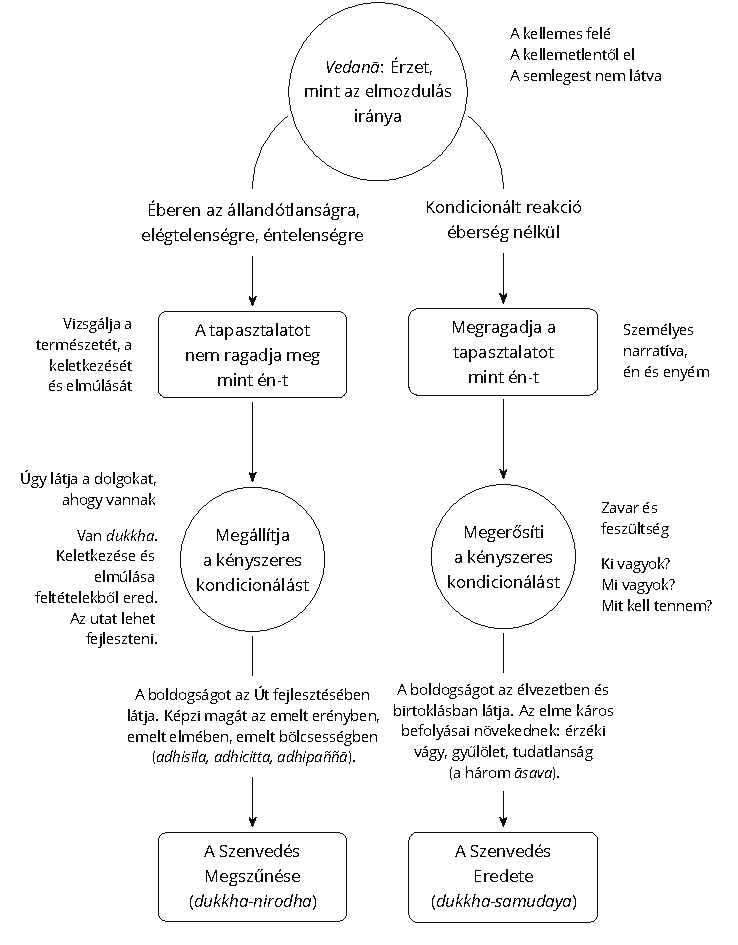
\includegraphics[width=\linewidth]{./manuscript/tex/diagrams/feeling-identification-hu.pdf}
\vspace*{\baselineskip}
\end{figure}

\clearpage
\normalpagelayout

Mi lenne, ha egy nap úgy ébrednénk fel, hogy semmire sem emlékszünk a
múltból? A tapasztalatunkat ilyen állapotban is megragadnánk, mint
\emph{én és enyém}. Annyira kiborító lehetne, hogy félelemtől bénulva
feküdnénk amíg meg nem tudunk ragadni valamilyen történetet, ami
megmagyarázza hol és kik vagyunk. Nem is kell elveszíteni a memóriánkat,
hogy ezt megfigyeljük: utazás közben lekésni egy fontos csatlakozást is
elég ijesztő lehet, hogy így érezzük magunkat, vagy más alkalommal
amikor nem tudjuk a helyzetünket irányítani.

Alázatra késztet mikor észrevesszük, mennyi mindent személyes ügynek
tekintünk, pedig észszerűen gondolkodva tudjuk, hogy nem kellene. A
Buddha azt tanítja, hogy az elme továbbra is az `én és enyém' képzetét
alkotja az érzékek tapasztalatából, amíg ennek a tapasztalatnak a
mulandóságát nem értjük teljesen. Személyes ügynek tekintjük és meg
vagyunk győződve, hogy vagy (1) `Ez én vagyok', (2) `Én ebben vagyok',
(3) `Én ezen kívül vagyok', (4) `Ez az enyém', vagy (5) `Én örömöt
találok ebben'.\footnote{\href{https://a-buddha-ujja.hu/mn-1/hu/pressing-lajos}{MN
  1}, A létesülés gyökeréről szóló tanítóbeszéd}

Jaj, szegény elménk, miért nem vagyunk bölcsebbek? Kezdhetjük azzal,
hogy kevés figyelmünk jut másra, miközben szokás szerint azzal vagyunk
elfoglalva, hogy arról gondolkodunk hogyan kapjuk meg amit akarunk, és
arról panaszkodunk, amit nem kaptunk meg.

Mikor az érzék-kapu kontaktusba kerül egy érzék-tárggyal, ha jelen van a
figyelem, a tapasztalatot a három érzés (\emph{vedanā}) közül egyikként
érezzük, amit hasonlíthatunk ahhoz, hogy milyen irányba mozdulunk:

A kellemes felé, el a kellemetlentől, vagy békében maradunk a
semlegessel. A képzetlen elme gépiesen követi ezeket a megalapozott
mintákat és a mögöttesen húzódó hajlamok magukkal sodorják: a
szenvedély, gyűlölet és tudatlanság.

Ebben a tekintetben, az ember akkor érti az érzéseket, amikor érti az
érzékek kontaktusát. Ennek eredménye, hogy az ember a kellemeset
fájdalmasnak látja (mivel végső soron elégtelen a természete), a
fájdalmasat tüskeként látja (amit el kell távolítani, vagy türelemmel
elviselni), és a semlegeset állandótlannak látja (nem ringatja magát
tudatlanságba).

Ez magában foglalja, hogy nem gondol rájuk úgy, mint `én és enyém'.
Megismerjük őket, de a tudás nem lesz a \emph{miénk}. Nem tartoznak egy
személyhez, \emph{akié} az érzés.

\begin{quote}
Teljesen megértve az érzéseket,\\
Megtisztul még ebben az életben.\\
A Tanban szilárdan áll: a test széthullásakor,\\
A tudás mesterét sehol sem találni.

\bigskip

\quoteRef{%

\href{https://suttacentral.net/sn36.5/en/bodhi}{SN 36.5}, Látni kell

}
\end{quote}

\keywords{gondolkodás, leterhelve, érzekek visszafogása}

Sokat gondolkodhatunk erről, de ha analitikusan próbáljuk megérteni,
csak a fejünk fog megfájdulni. Ezt a megértést a testen keresztül kell
fejleszteni: egy jó kezdőpont az érzékek visszafogásának gyakorlása.

Figyelmesen őrizzük az érzék-kapukat. A tiszta éberség megtart egy
teret, egy kis távolságot a tudatosságunk és annak tartama között.
Amikor egy formát látunk, hangot hallunk, stb., nem ragadjuk meg a
tapasztalatot, sem mint ahogy egészben látjuk, sem egy-egy adott
jellemzőjét amit kedvelünk vagy nem. Lehet, hogy kedveljük a
tapasztalatot, de nem válunk tőle mámorossá. Lehet, hogy visszataszító a
tapasztalat, de nem húzzuk fel magunkat és nem válunk haragossá tőle.
Figyelmünk egy részét a lélegzeten tarthatjuk, vagy fenntarthatunk egy
tágas tudatosságot a test egészére -- ez segít támpontot találni, egy
biztos alapot, ami a bölcsesség készségünket informálja. Ha nem a
lélegzetre figyelünk, az is jól beválik, ha a pillanatnyi tevékenységünk
egy aspektusát figyeljük, mint amilyen a toll érintése írás közben, a
talpunkon érzett nyomás a padlón, vagy a test más érzetei.

Ez a testen alapuló gyakorlat egyszerűbb, mint intellektuális
megközelítés. Összegyűjti a mentális erőnket, és egy természetes
ritmusnak megfelelően, vagy csendes nyugalom, vagy figyelmes vizsgálódás
követi.

Észrevesszük, hogy képesek vagyunk megállni, és ami most velünk van, az
is elegendő. Gondolj arra, mit használtál a mai nap, tárgyakra és
információra is tekintettel? Lehet, hogy sok dolog van a tulajdonodban, de
egy napra egy kevés is elég. Nincs szükségünk annyi mindenre mint ahogy
gondoljuk, és lemondani róla nem veszteség, hanem egy teher alóli
felszabadulás. Ebben a visszafogottságban erőt és energiát találunk,
amit korábban a szétszórt vágy emésztett fel. A visszafogottság mindig
kéznél van, és nem veszélyeztetik külső tényezők.

Olyan ez, mikor megtanulsz kevesebbet pakolni a hátizsákodba egy túra
előtt. Némi tapasztalat után, nem is érted, miért kellett annyi mindent
cipelned korábban. Az erény olyan tettekből áll, amik boldogsághoz
vezetnek, és az erényt önmagunk felé is fordíthatjuk: a lemondás éppen
egy ilyen személyes erény. A megértés információval látja el az erényt,
és a boldogság, ami ebből születik, ebbe a megértésbe vetett bizalmat
erősíti.

\keywords{ānāpānasati, érzékek kontaktusa, érzetek, érzés}

A légzést figyeljük, és az érzékek működését. A szem formákat lát, és
megjelenik egy érzet. A fül hangokat hall, a test szilárdságot, hideget
és meleget érzékel. Ha van kontaktus az érzék-kapu és érzék-tárgy
között, megjelenik az érzet. A folyamat nem rajtunk múlik, ha van
kontaktus, nem választhatjuk, hogy ne jelenjen meg az érzet. Amikor a
kontaktus az érzék-kapu és érzék-tárgy között megszakad, megszűnik az
érzet. A jelenség a kontaktustól függően keletkezik és múlik el -- ebből
állt a tapasztalatunk. A mozdulatainkat irányíthatjuk, de ezen túl a
tapasztalat folyamatába nincs beleszólásunk: nem rólunk szól.

Amikor ezt nem vesszük észre, úgy gondoljuk a miénk az érzés. Ha az
érzettel jó érzés jár, azt várjuk nyerni fogunk belőle valamit, és ezért
ragaszkodunk hozzá. Az ilyen helytelen megértés húzódik a szükség és
nyugtalanság érzése mögött. Amikor csalódunk az elvárásainkban,
hajlamosak vagyunk feltenni, hogy mi rontottuk el valahogy, vagy valaki
más hibája volt. Egy másik élményt kezdünk keresni, ami majd megfelelőbb
lesz, és azt reméljük ez az új élmény nem így fog lejátszódni.

\enlargethispage*{2\baselineskip}

Az érzékek kapcsolatát így figyelve, az érzések már nem vonzóak vagy
visszataszítóak. Látjuk, hogy egyik hajlam sem lesz stabil és
megbízható. Ez nem tompaság. A meditációban a tapasztalat felé
fordulunk, nem attól el. Ehelyett egy érzékeny, higgadt figyelmet
fejlesztünk. Éberek és érzékenyek maradunk a tapasztalatra, de az már
nem irányít, és nem kavar fel minket. Nyugodtak maradunk.

\clearpage
\figurepagelayout

\begin{figure}[h]
\caption{Érzék-Kapcsolat és Érzet}\label{fig-sense-contact-feeling}
\bigskip
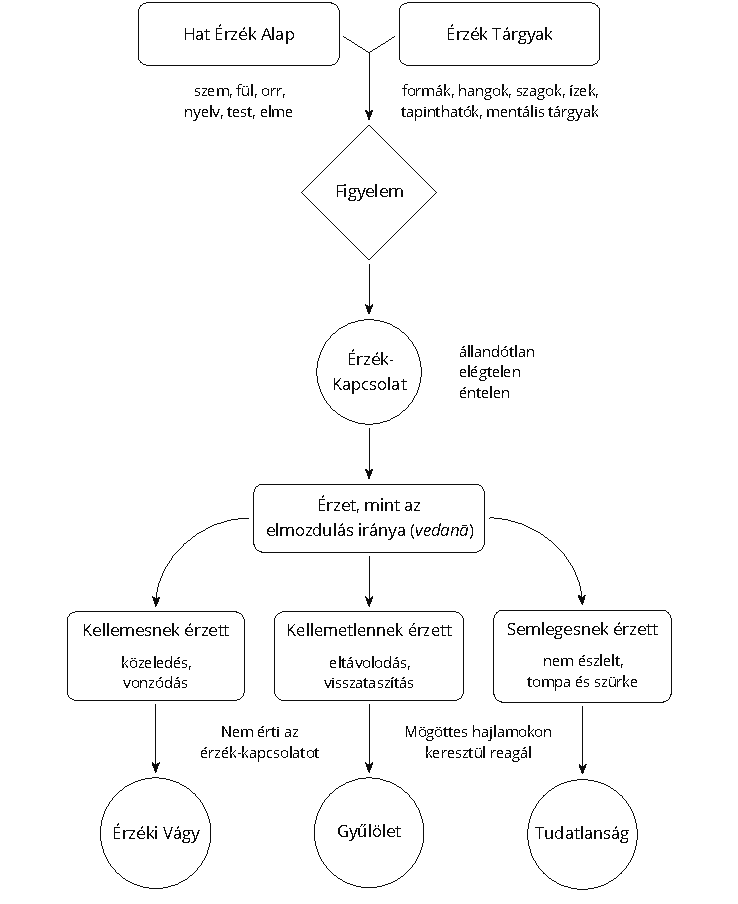
\includegraphics[width=\linewidth]{./manuscript/tex/diagrams/sense-contact-feeling-hu.pdf}
\end{figure}

\clearpage
\normalpagelayout

\vspace*{-\baselineskip}

\keywords{önnarratíva, elbeszélés}

Milyen hatással van ez arra, ahogy elbeszéljük magunknak a
tapasztalatainkat? Azt mondjuk magunknak, hogy ez az érzés jó volt vagy
rossz, és mit kellene erről gondolnunk. Egy központi eleme ennek a
narrátori szövegnek a \emph{mi érzéseink}, jellemzően abban az irányban,
hogyan legyen több a jó fajtából.

Mi történik, mikor észrevesszük, hogy mind a jó és a rossz tapasztalatok
instabilak, megbízhatatlanok, és a keletkezésük és elmúlásuk nincs az
irányításunk alatt? A belső értékeink átrendeződnek,
a vágy helyett a mulandóság által vezérelve.

\keywords{változékony természet, bölcs vizsgálódás}

Rendszerint akkor kezdünk csak figyelni, amikor észrevesszük, hogy
valami rossz, valami fáj, valami miatt szenvedünk. A kellemes
tapasztalatokra nem igénylünk annyi magyarázatot, ugye? Ezt a frusztrált
érzést, elégtelenséget és terjengő gondolkodást jelként használhatjuk a
magunk számára, hogy kezdjünk éberen vizsgálódni.

Gondolatban lépj egyet vissza, és figyeld a tapasztalatot mint egy
folyamatot, aminek van eleje, változáson megy keresztül, és megszűnik.
`A testben hol érzem ezt az érzést? Emlékszem, mikor kezdődött? Tudom
figyelni, ahogy változik? El tudom kapni, ahogy az érzés megszűnik?'

Nem tudjuk irányítani a világot magunk körül, de a hozzáállásunk
befolyásolja, mit látunk szabad választásként. A szemléletünk nyitja meg
vagy zárja be az ajtókat a tettek felé, amiket lehetségesnek látunk.
Ezek a tettek hozzák létre a helyzetet, amiben élünk, és befolyásolják,
ahogy a helyzetben látjuk magunkat. Ha nem vizsgáljuk a tapasztalataink
természetét, hajlamosak vagyunk a jó érzéseket jutalomnak és a rossz
érzéseket büntetésnek tekinteni, ennek folytán az életünk értelme ezek
körül fog forogni. A belső világunk mindig azokról a kérdésekről fog
szólni, mint: `Ki vagyok én \ldots{} Hogyan tegyem \ldots{} Miért kell
tegyem \ldots{} Mit kellene tennem \ldots{}' Nem olyan terhes érzés ez,
amit jobb lenne elhagyni?

Az alapos és felületes vizsgálat a \emph{szuttákban}\footnote{\href{https://a-buddha-ujja.hu/mn-2/hu/forizs-laszlo}{MN
  2}, Az összes káros folyamatról szóló tanítóbeszéd} használt
kifejezés, mely különbséget tesz a felületes figyelem között ami növeli
a zavarodottságunkat, és az alapos figyelem között ami tisztánlátáshoz
és helyes megértéshez vezet. A felületes vizsgálat átsiklik az
állandótlanság, elégtelenség és nem-én jellemzői felett, így mindent a
saját ügyének tekint. Az alapos vizsgálat felismeri az érzéki
tapasztalat jellemzőit, és a Négy Nemes Igazsággal összhangban
elmélkedik róluk.

\keywords{ragaszkodás az énhez, karóhoz kötött kutya, vizsgálódás}

Emlékszel, hogy egy kutya, pórázzal kikötve egy karóhoz, hogy futkos
körbe-körbe a karó körül? Ül, áll, járkál vagy futkos körülötte, de
minden amit tesz, a karó körül teszi.\footnote{\href{https://suttacentral.net/sn22.100}{SN
  22.100}, Póráz} Az ego által vezérelt gondolatok kavargása is ilyen.
Lehet, hogy elfoglaltan tart minket, de továbbra is ragaszkodunk a
középen lévő énhez, nem vagyunk képesek sehova máshova menni. A póráz az
azonosulás és megragadás (\emph{upādāna}), az a folyamat, ami kialakítja
az `én és enyém' képzetét az érzékek tapasztalatában, vagy akörül,
melynek alapvető igazság szerint nincs semmi ilyen jellemzője. Ez vezet
minket a felületes vizsgálathoz, arra összpontosítva kik vagyunk, mi
lesz velünk, növelve a kétségünket és zavarodottságunkat.

Az `én és enyém'-ben gyökerező kérdések csapdák. Egyre tovább
húznak-vonnak minket anélkül, hogy szabadsághoz vagy megálláshoz
vezetnének. Ha azt vesszük észre, hogy ki vagyunk kötve egy karóhoz, mit
tegyünk? Elvágni a pórázt jó ötletnek tűnik.

A meditáción belül értelmezve, a vizsgálódásra nem mindenféle
gondolkodás alkalmas. Nem minden fajta gondolat fog belátást
eredményezni. Vizsgálódó meditáció közben, a tapasztalatunkat ok-okozati
folyamatra bontjuk le, amire a Négy Nemes Igazságot\footnote{\href{https://a-buddha-ujja.hu/sn-56.11/hu/farkas-pal}{SN
  56.11}, A Tan kerekét forgásba hozó tanítóbeszéd} használjuk
útmutatóként.

Ez egy olyan tapasztalattal kezdődik, amit személyesen könnyű
azonosítanunk: a szenvedés, feszültség, elégtelenség, avagy Páli szóval
\emph{dukkha}. A gondolat iránya nem \emph{az én szenvedésem}, mint
személyes történet, hanem személytelen, természetes folyamatként
szemléljük azt.

\keywords{dukkha}

A kezdő álláspont azt elismerni, hogy a feszültség, a szenvedés
\emph{itt} van. Ez ismeretként triviális, hogy igen, van a világban
feszültség és szenvedés. De amikor magunk tapasztaljuk, szeretünk mégis
inkább valami másra figyelni, vagy hajlamosak vagyunk valakit hibáztatni
érte. Ezerféle dolgot teszünk, csak ne kelljen tudatosan elismerjük és
érdemben foglalkoznunk vele.

Az utasítás itt az, hogy csak az fog előre vezetni, ha a szenvedés felé
fordulunk, és azt vizsgálva keressük a megértés módját. A Buddha
tanításában ez az Első Nemes Igazság: van szenvedés, és a nemes
hozzáállás az, ha felé fordulunk és megértjük.

Mit értünk meg? Azt, hogy a szenvedés nem a semmiből jött létre, hanem
korábbi tényezők eredménye. Ha így tudjuk vizsgálni a helyzetet, nem
vagyunk tehetetlenek. Még ha nem is értjük a helyzetünk minden apró
tényezőjét, már az is megkönnyebbülés, hogy talán tudunk valamit
változtatni.

\keywords{a dukkha eredete}

A Második Nemes igazság arra mutat rá, hogy a szenvedést kiváltó okot
magunkban találjuk. Ez a kívánságunk, hogy a tapasztalataink másképpen
legyenek mint ahogy természetüktől fogva vannak. A görcsös
ragaszkodásunk ahhoz, ami állandótlan, törékeny, és nem megtartható. A
szenvedés, a \emph{dukkha} amit tapasztalunk, ettől a ragaszkodástól,
szomjas vágytól függ. Az utasítás, a nemes hozzáállás itt az, hogy ezt a
szomjas vágyat és ragaszkodást el kell engednünk, mert a mulandó
élményekhez való ragaszkodás szenvedés.

\keywords{a dukkha megszűnése}

A kiváltó ok megszűnésével megszűnik az eredmény, a szenvedés is. A jó
hír, hogy a szenvedés végét is magunkban találjuk.

Ebből a szemszögből láthatjuk, hogy az elme hozza létre azt a fajta
világot, amiben élünk. Ha figyeljük, van esélyünk, hogy legalább ne
rontsunk a helyzeten. És ki tudja, akár még javíthatunk is rajta?

A Harmadik Nemes Igazság erre irányítja a figyelmünket: van megoldás,
nem kötelező keserűségben és értelmetlen küszködésben élnünk. A tanács,
a nemes hozzáállás az, hogy gyakoroljunk és tapasztaljuk ezt meg a
magunk számára, a megértésen és a ragaszkodás elengedésén keresztül. Így
lehetővé tesszük a szenvedés megszűnését.

\clearpage

Még ha nem is tudjuk rögtön elengedni, már az is megkönnyebbülés, ha
látjuk az összefüggést: `Ha elengedném, nem szenvednék tőle'.
Ez már a munka fele. Egész eddig térkép nélkül bolyongtunk, de innen már
van út előre.

\keywords{a gyakorlás útja}

A Negyedik Nemes Igazság az út gyakorlását írja le. A Buddha nyolc
tényezőre bontotta, melyek magukban foglalják a mindennapi élet
helyzeteit és a meditáció fejlesztését is.

A Nyolcrétű Ösvény részei a (1) megértés, (2) szándék, (3) beszéd, (4)
tett, (5) megélhetés, (6) erőfeszítés, (7) éberség és (8) elmélyülés.
Amikor egy tényező összhangban van az igazsággal, \emph{helyesnek}
nevezzük: Helyes Megértés, Helyes Szándék, és így tovább. Az utat
részekre bontani segíti a vizsgálódást, könnyebb ilyen módon
gondolkodnunk, de az út tényezői nem különállóak: egymást erősítik és
támogatják. A gyakorlás egyesült egészként valósul meg.

Amikor leginkább szükségünk van a gyakorlásra, az \emph{azonnal} kell.
Nem állhatunk meg tényezőket számolni. Olyan eszköz hasznos, ami
hordozható és könnyen elérhető egy adott helyzetben. Mikor olvasunk,
töprengünk a jelentésen, van időnk körbejárni a szavakat, ez a tanulás
szakasza. Viszont az éber figyelem, mint elvont ötlet nem sokat használ
-- akkor értékes, ha gyakoroljuk, mikor kéznél van a jelen pillanatban.

\enlargethispage*{\baselineskip}

Mindig ide térünk vissza. Emlékszünk a múltra és tervezzük a jövőt, de
az emlékezés egy jelen tapasztalat, a tervezés egy jelen tapasztalat. A
meditáció gyakorlását nem a jövőért végezzük. Ha a megértést,
szabadságot, boldogságot, akadályok túllépését egy jövőbeli állapotként
látjuk, ezzel csak több lesz a terhünk. Az elengedés a jelenben
történik, ahol az állapotok nélkülünk változnak.

\chapter{Ciklusok}

\keywords{lépések a gyakorlásban, leírások és tudatosság}

\noindent A meditáció a jelenbeli érzéseken, tapasztalatokon keresztüli
megismerést tanítja. Az utasítások lépésről-lépésre írják le a
fejlődést, de a jelenben csak egy pillanat elérhető számunkra. Előre
vagy hátra lépünk? Bármely irányban, a tapasztalat egyszerre egy lépés,
a lépés ahol minden változik. Szavakat használunk, hogy leírjuk a
tapasztalatot, de a tudatosság erre a tapasztalatra szótlan. Az éber
figyelem aktívan befelé néz, mintha önmagát kérdezné, de nem vár
választ. A nyelv szimbólumai is korlátozóak. Rögzített reprezentációkból
állnak, míg a tapasztalat mozgásban van.

A meditáció célja nem az utasítás lépéseinek tökéletesítése. A cél a
jelen tapasztalat tiszta ismerete, ami visszaállítja a helyes
nézőpontot. Kialakulhat bennünk az a benyomás, hogy mindig ugyanazt a
lépés sort kell teljesítenünk, és amikor az elme nem aszerint a sorrend
szerint fejlődik, csalódottak vagyunk.

\keywords{narrátor elme, tapasztalat mint alap, a megfelelő festéket választani}

És ami még rosszabb, úgy látszik mások békésen meditálnak, ők biztos jól
értik! A gyakorlás felszínre hozza az önkétséget. Vizsgálhatjuk ezt a
másik oldalról: Valaki talán dicsér minket, `Olyan békésnek tűntél, te
biztos tudsz valamit!' De mi tudjuk milyen szétszórt gondolatokkal volt
tele a fejünk, láthatjuk milyen megbízhatatlanok az ilyen benyomások.

A narrátor elme gépiesen folyton megjegyzéseket tesz, de nincs mögöttük
mélység vagy vizsgálódás. Érdemes egy lépés távolságból nézni ezt, és
megízlelni milyen megbízhatatlan és bizonytalan a saját gondolkodó
elménk, még ha azt is gondoljuk, `Ebben biztos vagyok!'

Fordítsd meg ezt a hozzáállást és kezdd a tapasztalattal. Egy kérdező,
kíváncsi figyelemmel indulj neki, ami szótlanul érdeklődik a jelenről.
Ha a tapasztalatunkat vesszük az alapnak, ahogy ez a tapasztalat most
van, az milyen megértést ad nekünk?

Először magunkat vesszük szemügyre -- Hogyan érezzük magunkat? Milyen
állapotban vagyunk? -- erre válaszolunk intelligensen, a meditációnk
megfelelő irányba való fejlesztésével. Amikor falat festünk, először a
falat vesszük szemügyre, kiválasztjuk az annak megfelelő festéket, és
\emph{azután} követjük az utasítást a dobozon. A rossz fajta festék le
fog peregni, nem igaz? Van amikor le kell higgadnunk, máskor energiát és
erőfeszítést kell bevetnünk, vagy várni, hogy a belső vihar tovább
álljon.

A meditáció különféle módszereinek lépései az imitáción keresztül való
tanulás része. Egy példát követve figyeljük önmagunkat és meglátjuk
hogyan működik az elménk. Amikor szenvedést érzünk, vagy fel tudjuk
oldani, vagy türelmesen kivárjuk, amíg véget ér. Később tiszta fejjel
visszanézünk, tudjuk mi történt minek a hatására, és a gyakorlásra
irányuló megértésünk nőni fog. Ebből tanultunk valamit, és nem
ragaszkodunk az első, bemutató példa részleteihez.

\keywords{fejlődés ciklusokban}

Ez egyszerű lenne, ha a meditációnk egyenes vonalban fejlődne, a
gyakorlással töltött percek és órák számával egyenes arányban. Azt
tervezzük, hogy le fogunk ülni, az elején kissé szétszórtan, de egy
órával később, \emph{ha jól tudunk meditálni}, nyugalmat fogunk érezni,
az elménk tiszta és összeszedett lesz. Legalábbis erre számítunk.

Később vissza emlékezünk mi történt a meditáció alatt, és azt látjuk,
hogy nem ez szokott történni. A tapasztalatunk nem egyenes vonalban
fejlődik a sekélytől a mélyig, vagy a szétszórttól az összeszedettig.
Azt gondolhatjuk, ez a mi hibánk, mert `nem vagyunk jók' a meditációban,
vagy `nem helyesen' követjük a lépéseket.

Amit megpróbálunk terv szerint, lépésről lépésre követni egy módszert,
minden az elvárásainktól eltérően történik. Arra gondolhatunk, `Talán
nem próbálom elég erősen?' Egyre jobban neki feszülünk, és egyre
fájdalmasabb lesz. Ilyen az az érzés, amikor egy véleményt rá akarunk
erőltetni a tapasztalatra.

Ha felidézzük, hogy a tapasztalatunk hogyan változik idő közben, más
mintát látunk. Egy tapasztalat megjelenik, változáson megy keresztül,
elmúlik, és egy újabb tapasztalat jelenik meg. Az elme ilyen ciklusokban
fejlődik, és ezek a ciklusok nem vesznek tudomást a céljainkról, hogy a
meditációnkat úgy akarjuk fejleszteni mint egy ranglétrát. A kommentáló
elme próbál egy személyes történetet illeszteni a tapasztalatra, arról,
hogy mi valaki olyan vagyunk, aki jó vagy rossz a meditációban.

Ehelyett vegyük a tapasztalatot alapigazságnak, és onnan induljunk.
Milyen fajta tapasztalat ez itt? Észrevehetjük, hogyan mozog a figyelem,
mint a tudatosság egy folyamata, hogyan megy keresztül különféle
ciklusokon.

Eleinte az elme elégedett az üléssel, ellazult figyelemmel pihen, mint
amikor egy séta után leülünk egy padra: ülni és lélegezni a béke
teljessége. De gondolatok jelennek meg és követjük őket. Megállunk, újra
nyugodtak és csendesek vagyunk, a gondolkodás lehet, hogy meg is áll
anélkül, hogy észrevennénk, hogy nem gondolkodunk. De a figyelem elkezd
mozogni, és megint észrevesszük magunkat, hogy gondolkodunk. Emlékek,
vágyak, nyugtalanság jelenik meg és észrevesszük, hogy ezen dolgoznunk
kell. Ezután az elme újra nyugodt, és visszatér a csendesség érzéséghez.

\keywords{tudás és megismerés, névadó folyamat, a tudás nem a miénk}

Némi ismeretre szükség van, de egy kevés is elég. A Buddha tanítására
emlékezni olyan kincs, ami nem fogy ki. A belátások és megértés viszont
nem válik a \emph{mi tudásunkká}, mintha az attól fogva a tulajdonunk
lenne. Az igazságot nem tehetjük egy dobozba, hogy eltárazzuk a
következő alkalomra, ehelyett folyamatosan felismerjük azt a jelenben.
Amikor rögzített elképzeléseket hozunk létre arról, amiről úgy gondoljuk
ezt már tudjuk, a gyakorlásunk elveszíti a kapcsolatot a valósággal.
Minden alkalommal újból az elejénél kezdjük, és onnan, bízunk a jelen
megismerésében.

A gondolkodó elme vonzódik a tényekhez és megállapításokhoz, egyfajta
biztonságot érzünk abban, ha tényeket tudunk felmondani. Szeretnénk
megállapítani, hogy `ez jó meditáció volt, ez rossz meditáció volt'.
Különbséget akarunk tenni és nevet adni a tapasztalatnak.

Ilyen az elégedetlen elme. Valamivé válni akar, meg akar érkezni egy
állapotba és nevet akar magának. De sehol nem szeret megállni. Megy
tovább és tovább, amíg csak észre nem vesszük, hogy a folytonos futásban
teljesen kimerültünk.

Amikor a tudatban láthatóvá válik, hogy mi magunk tesszük ezt, a
névkeresés megáll. Megáll, mert a látás felváltotta a nem-látást; a
tudás felváltotta a tudatlanságot. Tudatosan látni a névadó folyamatot
elegendő, hogy megtörje a kényszert a folytatásra.

A jelenben minden változik, semmi sem rögzített. Minden mozog, a
tapasztalat erre-arra fordul és folyik. Nem áll meg egy fotóra és vár
amíg nevet adunk neki. Ebben a változásban, a kétséggel és aggodalommal
teli kérdések, az önazonosság és a célok elvesztik a jelentésüket. A
\emph{Mahāsatipaṭṭhāna Szutta} kifejezését használva: `\emph{Szabadon
időzik, semmihez sem kötődve a világon}.'\footnote{\href{https://a-buddha-ujja.hu/mn-10/hu/toth-zsuzsanna}{MN
  10}, Az éberség megalapozásáról szóló tanítóbeszéd}

Ennyi elég, így ismerve az elmét megállunk és megérkezünk egy helyre,
ahol hálásak tudunk lenni a létezésért. Nem egy különös dolog miatt.
Hálásnak lenni, hogy van tapasztalat, megismerés, tisztánlátás, és a
szabadság, ami engedi, hogy megálljunk és nem kell több és több felé
mennünk.

\keywords{határozatlan vonalak, korlátozott szimbólumok, megismerés névadás nélkül, érzések határvonalak nélkül}

Kiegyensúlyozott testtartásban a test kifinomult belső érzéseit könnyebb
megfigyelni. Befelé irányítjuk a figyelmet, kíváncsi hozzáállással. Nem
tudjuk előre mit fogunk találni.

Megjelennek a test érzetei, illetve az érzések, amik a megismerésükhöz
társulnak. Megtapasztaljuk őket, de gyakran nincsenek tiszta
határvonalaik. Nincsenek éleik, vagy határozott formájuk. Próbálunk
szavakat találni rájuk, de ezek nem illeszkednek jól. Nem vagyunk
biztosak abban, hogy minek nevezzük őket.

\enlargethispage*{\baselineskip}

Minden szimbólum, amit névként használhatnánk, hiányos. A nyugati
kultúránkban erősen bízunk a tényekben, és szeretünk visszatérni ahhoz a
biztonsághoz, amit a nevekben és terminológiában érzünk. Nem ismerősek
számunkra azok a tudati folyamatok, amik nem használnak neveket és
rögzített szimbólumokat. A megfigyelt érzések, a tapasztalat maga nem
tisztán meghatározott, de mégis tudjuk, hogy jelen van ez a tapasztalat.

Így meg tudjuk különböztetni a nevet adó folyamatot magától a
tapasztalattól. A test kifinomult érzései ködszerűek, nincsenek éles
határaik. Belégzés és kilégzés közben, megtapasztalhatjuk milyen ez az
érzés az egész testben -- mindenhol egyszerre. Az egész test lélegzik.
Van érzés és tapasztalat, de nincsenek nevek és éles határok.

A nevet adó folyamatot elhagyjuk, és észre vesszük, hogy képesek vagyunk
ismerni ezeket az érzéseket, ahogy jelen vannak. A megismerő elme örömét
találja abban, hogy szűrők nélkül szélesebb körben fogja be a
tapasztalatot. Tudjuk, hogy milyen a tapasztalat, anélkül, hogy nevet
kellene találnunk rá.

\keywords{az elme vizsgálata, túl sok gondolkodás}

A kártékony elmeállapotok érzetében észrevehetünk egyfajta hőséget,
nyugtalanságot, elégedetlenséget és szorongást. Emlékezünk, hogy
türelemmel forduljuk felé, és fenntartsuk a kitartást az állapot
érzéseinek jelenlétében. Ez is meg fog változni, ez is el fog múlni, és
meg tudjuk ezt várni. Amikor tudjuk hol állunk, a legtöbb esetben ennyi
elég. Az elme folyamatai maguktól meg fognak változni. Ha nem teszünk
tüzelőt a tűzre, az el fogja égetni amije van és magától kialszik.

Az elhatározás és ismétlés része a gyakorlásnak, de egy kifejezett cél
felé törekedésben az erőfeszítés keserűvé és fárasztóvá válik. `Ez már a
teljes felébredés? Vagy legalább egy része? Mikor fog már szólni a
meditációs harang?' Ne~egy állapotot keress. Az elme, ami felébredetté
akar válni, túlbonyolítja a helyzetet.

A jelen tapasztalat mindig egyszerű, az éber figyelemnek megvan a
képessége a bölcs megértésre. A gyakorlásban folyton ehhez térünk
vissza, ez irányítja az erőfeszítést.

Ezt nem erőltethetjük akarattal, és nem garantálhatjuk mi fog történni:
bíznunk kell a folyamatban. Ami marad, az a jótékony elme ami érti mi
történik. Nem sürget minket a kényszer, és nem kell végig erőltetnünk
magunkat a dolgokon. A nehézség után van terünk ahhoz, hogy megjelenjen
a hála, és értékelni tudjuk a könnyedség hűs, kényelmes érzését.

\keywords{beépített gyakorlás}

A tanítóinkra nézünk fel példaként. Nem azért meditáltak, hogy elérjenek
egy különleges állapotot és azután keressenek valami más tennivalót. A
meditáció nem elkülönült, hanem beépült az életükbe. A \emph{szutták}, a
buddhista hagyomány megőrzött szövegeinek példáiban, a Tiszteletreméltó
Száriputta az üresség szemléletét gyakorolta,\footnote{\href{https://a-buddha-ujja.hu/mn-151/hu/fenyvesi-robert}{MN
  151}, Az alamizsna megtisztítása} míg a Buddha a jeltelenre irányuló
koncentrációt tartotta fenn. Így folytatták a meditációt.

\chapter{Csónak}

\keywords{sétáló meditáció módszere}

\noindent A sétáló meditáció egy energikusabb alternatíva az ülő
testtartás mellett. Keress egy ösvényt, vagy egy kis területet, ahol van
elég hely megtenni néhány lépést, oda-vissza séta közben. Habár
sétálunk, a figyelmünket befelé irányítjuk. Nem egy bizonyos helyre
sétálunk. A sétáló testtartást használjuk az elme fejlesztésére.

Egy kültéri, magányos helyszín az ideális, de beltérben, egy nagyobb
szoba is megfelelő.

Válassz két pontot, ami között tisztán járható út van. Ez lehet két fa,
vagy akár két bútor is. Egy rövid ösvény vehető tizenöt lépés hosszúnak,
egy hosszabb lehet harminc lépés is. Állj meg az ösvény egyik végén, és
indulj el lépésenként, figyelmesen a másik végéhez, tisztán elhatározott
szándékkal arra, hogy a meditáció tárgyával maradsz, mint például a
lélegzet, vagy a mozgó test fizikai érzetei. Irányítsd a tekinteted
lefelé, nézz magad elé néhány lépésnyire. Az ösvény másik végén állj
meg, és várj pár lélegzet vételnyi időt. Tartsd a figyelmed elmélyedve a
meditációban, fordulj meg, és kezdj el sétálni a másik irányba.

Tartsd a kezed úgy, hogy segítsen fenntartani a folyamatos belső
figyelmet. A legtöbben összefogják a két kezet maguk előtt. Nem a kezek
pontos helyzete számít, de ha oda-vissza lengeted a karjaid, az könnyen
eltereli a figyelmed.

\clearpage
\thispagestyle{empty}\mbox{}
\photoFullBleedPlaceholder{%
  TODO: Illustration of walking meditation.%
  \illustration{Sétáló Meditáció Testtartás}%
  \label{illus-walking-meditation}%
}
\clearpage

Igazítsd a séta sebességét az energia szintedhez és a meditáció
tárgyához. Egyesek gyors és határozott lépésekkel gyakorolják a sétáló
meditációt, mások lassú és óvatos lépéseket tesznek. A megfelelő
sebesség akár egy alkalom időtartamán belül is változhat. Tapasztald meg
a különféle változatokat és találd meg azt, ami illeszkedik a
gyakorlásodhoz és mentális hátteredhez az adott helyben és időben.

\keywords{az érzések manipulálása, fontoskodás}

Korábban, a sétáló meditációtól csak még feszültebb lettem. Úgy
gondoltam hasznos, de a módszer elég határozatlan volt, és nem voltak
pontos részletek arról, hogyan is kellene azt végezni. Úgy éreztem, egy
pontokba szedett listára van szükségem, amin végig mehetek és
ellenőrizhetem, jól végzem-e a feladatot vagy sem.

Folyton el akartam sétálni egy \emph{másik helyre}, ahol majd
\emph{máshogy érzem} magam. Elkezdtem a sétáló meditációt két fa között,
de úgy éreztem mintha nem lenne semmi hatása, és folyton változtattam a
séta módját, hogy manipulálni tudjam hogyan érzem magam. `Lépkedj
gyorsabban, az használni fog. Lassíts le, és összpontosíts. Próbálj így
lélegezni, és úgy lépkedni, amíg máshogy nem érzed magad.'

Az is fontos volt, hogy mások lássák, valami fontos dolgot csinálok.
Addig járkáltam oda-vissza, amíg a füvön elkezdett látszódni a
kitaposott ösvényem. Ez volt a bizonyíték: 'Itt van, látom, hogy tettem
valamit, és \emph{mások} is láthatják!

Látható, hogy az ilyen küszködést mennyire az a kérdés vezérli: `Hogyan
tudnám jobban érezni magam, magammal kapcsolatban?'

A motiváció az érzések \emph{manipulálása} körül forog, nem azok
\emph{megértését} keresi, hogyan keletkeznek és múlnak el. A fontoskodás
nem hasznos hozzáállás a gyakorláshoz. A vágyunk meghatároz egy külső
jelet, és szörnyen fontossá válik, hogy ezt lássuk, és, hogy mások
számára látható legyen. Az a \emph{fontos} ösvény a fűben amit a fűbe
tapostam (ami valószínűleg eltűnt a következő reggelre) egy példa erre.
Kifejezni ezt a magunk számára, amikor észrevesszük, hogy ez történik,
már önmagában megváltoztatja a hozzáállásunkat a folyamathoz.

Egy hasznos hozzáállás a gyakorláshoz az, ha úgy közelítjük meg, mintha
valami teljesen hétköznapi dolgot végeznénk, de ehhez hozzáfűzzük a
felfedezés szemléletét, és emlékezünk arra, hogy az értéke nem egy
világi cél, ebben nincs tét, amit megnyerjünk, vagy elveszítsünk. Az is
segíthet, ha \emph{csökkentjük} a meditáció idejét. Jó benyomást kelt,
ha három óra hosszat folyamatosan sétáló meditációval töltünk, de a
nyomás feszültséghez vezet. Mi a helyzet tíz perc meditációval? Lehet,
hogy nem világhír, de talán jó élmény és érdekes lesz.

\keywords{gondolatok megállítása, éberség a fejben, belső monológ, irányítás, hétköznapi gyakorlás}

A gondolkodás jellemzően erősödik és önmagunk körül forog, amikor úgy
tekintünk az éberségre, tudatosságra, vagy a meditációra, mint egy olyan
dologra, ami valahol a fejünkben történik. Abból a nézőpontból, az
éberség olyan dologgá válik, amit `nekem kell csinálnom az
agyamban'.\footnote{Cf. Chapter 4, `Mindfulness Mania' in
  \href{https://www.goodreads.com/book/show/44439993-why-i-am-not-a-buddhist}{Why
  I Am Not a Buddhist by Evan Thompson}} Ez alá becsüli az éberséget,
mintha csupán egy rongybaba lenne az agy bábszínházában. Habár ez a kép
illik a kedvenc elképzelésünkhöz, ami szerint mi irányítjuk a műsort, ez
a valóság egy szűk nézete.

A kognitív felfogásunk ennél egy sokkal összetettebb, a környezetet
magába foglaló folyamatok rendszere. Megfigyelheted, hogyan változik a
figyelmed, vagy az egész személyes hozzáállásod, például amikor egyik
épületből belépsz a másikba, vagy a belső térből a szabadba. A tested
reagál arra, hogy egy új környezetben vagy, a különféle szociális
környezet megváltoztatja a viselkedésed, nagyszámú belső és külső
tényezők vesznek részt abban, hogy létrehozzák az észlelést, amit úgy
tapasztalsz mint `az én elmém.' A felfogásunk, vagy elménk, magába
foglal egy hálózatban működő folyamatok együttesen működő rendszerét,
melyek a testünk széles környezetéből veszik a beérkező jeleket. Ahogy
többet tapasztalunk ebből történés közben, az derül ki, hogy nincsenek a
kezünkben a drótok, amiket meghúzva az elménk akaratunk szerint járja a
táncot.

A gondolkodó és érvelő elme egy eszköz, amit a minket motiváló célokra
használunk. Nem a `jó érv' motivál minket, hanem a motiváció miatt
keresünk jó érvet. Ne akarj a gondolatok végére jutni; vedd észre mi az,
ami motivál téged a gondolkodásra. Ha azt elengeded, a gondolkodást is
elengeded. A belső rágódással gyakran magunkat akarjuk vigasztalni úgy,
hogy elképzeljük, mintha lenne irányításunk egy bizonyos helyzetben;
vagy megpróbáljuk visszanyerni az irányítást valami olyasmi felett, ami
már megtörtént. Olyan ez, mintha az esőről gondolkodnánk: esni fog attól
függetlenül, hogy rágódunk rajta vagy sem.

Ha \emph{tudunk} tenni valami hasznosat a problémával kapcsolatban, az
megnyugtató. Ha nem tudunk, mert teljesen az irányításunkon kívül esik,
legalább ezt tudhatjuk, és felhagyhatunk a belső tépődéssel.

A gondolkodásnak gyakran egy élesen meghatározott szóbeli tárgya van.
Amikor a figyelmünk módját eltoljuk egy tágasabb, folyékonyabb
hozzáállás felé, az elme nem tud szavakat találni rá, és átváltunk egy
nem verbális, szótlan felfogási módba; a körülöttünk lévő világot ezen
keresztül észleljük.

A nem-gondolkodás úgy tűnhet mint valami misztikus állapot, mintha egy
magas fokú meditációs szint lenne. Nem szoktuk megkérdezni meditáló
társainktól mennyi belső párbeszédet használnak, ugye? Amikor
megkérdezzük az embereket, kiderül, hogy van aki egyáltalán nem folytat
magával belső monológot.\footnote{\href{https://www.psychologytoday.com/us/blog/pristine-inner-experience/201110/not-everyone-conducts-inner-speech}{Not
  Everyone Conducts Inner Speech (psychologytoday.com)}} Sokkoló
meglepetésként éri őket, amikor megtudják, hogy más emberek beszélnek
magukkal a fejükben. Mások csak időnként kezdenek belső párbeszédet, míg
megint mások folyamatosan, szünet nélkül ezt teszik. Ez egy érték skála,
mint egy tekerő gomb különféle állapotai. Személyesen hozzá vagyunk
szokva egy bizonyos mértékű belső párbeszédhez, de a szint, amin ezt a
mentális képességet használjuk egy szokás, amin állítani tudunk.

Ha séta közben úgy érzed, magával ragadott a gondolkodás, vedd tágabbra
a területet, amire tudatos vagy; hogy magába foglaljon egy szélesebb
kognitív mezőt. Idézd fel a nyugodt hallgatás hozzáállását, fordítsd el
a figyelmet a szemek és a fej környékéről más irányba.\footnote{Cf. page
  117, Gently Listening in
  \href{https://forestsangha.org/teachings/books/alert-to-the-needs-of-the-journey?language=English}{Alert
  to the Needs of the Journey by Ajahn Munindo (forestsangha.org)}}
Tartsd a szemeket magad előtt, alacsonyan a sétáló ösvényen.
Képzelheted, mintha minden irányba látnál a testeddel, vagy mintha az
ösvényt a talpaidon keresztül látnád, a tapintás és nyomás érzetein át.
Nyisd meg a figyelmed, hogy magába foglalja az egész testet, mint
egyetlen mozgásban lévő érzet. Nyisd a figyelmet még tovább, ki a sétáló
ösvény közvetlen környezetére.

Rövid meditációk, amik betöltik a céljukat, jobbak, mint hosszú
időszakok, amit azzal töltesz, hogy az óra állásán aggódsz. A cél nem
az, hogy több feszültséget keltsünk. A cél az elme tisztán látása és
nyugalma. Gyakorolunk, vele maradunk, így élünk abban a térben, ahol a
feszültség feloldódik.

\keywords{a tapasztalatok figyelése, érzékek kontaktusa}

A meditáció elején összegyűjtjük a figyelmünket azzal, hogy a légzést
figyeljük, vagy a séta közben tapasztalt érzéseket, lépésről lépésre.
Egy zaklatott, izgatott elmétől nem várhatunk éber és kiegyensúlyozott
intelligenciát, ezért lényeges megalapozni legalább némi nyugalmat.

Vizsgálódásra a nyugodt elme alkalmas. Mit tanulhat a boldog ember a
Buddha tanításából? Mit tanulhat a boldogtalan ember? Vagy, aki nem érzi
magát sem különösen jól vagy rosszul, éppen megvan ahogy van?

A tapasztalatunkat figyeljük, az állandótlanság jeleit, az érzések,
gondolatok kezdetét és végét, ahogy megjelennek, változnak és
megszűnnek. A magunk számára vizsgálódunk, ez ad a tanítások szavainak
jelentést és közvetlen hasznot.

Tapasztalataink az érzékeken keresztül nyilvánulnak meg. A szem formákat
és színeket fog fel, a fül hangokat, az orr szagokat, a nyelv ízeket, a
test a tapintás, a hideg és meleg benyomásait érzékeli, az elme pedig
észleli a gondolatokat, emlékeket és más mentális folyamatokat.

\keywords{három érzés, állandótlanság}

Az érzetek (\emph{vedanā}) három minőségben jelennek meg. Lehetnek
kellemesek, és vonzódunk feléjük; lehetnek kellemetlenek vagy
fájdalmasak, és inkább távolodnánk tőlük; vagy lehetnek semlegesek, és a
jelenlétük nem zavar minket. A semleges érzetek egy jellemzője, hogy
kellemessé válnak, ha figyelünk rájuk, mint a légzés.

A megjelenésük és elmúlásuk nincs közvetlen irányításunk alatt. Az érzet
szükséges feltételei a kapcsolat az érzék és érzék-tárgy között,
illetve, hogy a figyelmünk oda irányuljon. A kapcsolattal az érzet
magától megjelenik. Amikor a érzék-kapcsolat megszakad, vagy a
figyelmünk másfelé fordul, az érzet megszűnik.

A boldog ember, aki kellemes érzéseket tapasztal, tanulhat ezek
vizsgálatából. A vonzó benyomás arra vezeti minket, hogy ragaszkodjunk a
kellemes érzethez, ha elfelejtjük, hogy ez a függő állapot
megbízhatatlan. Az érzeteket nem birtokoljuk. Lehetetlen megtartani,
nincs mélyebb lényege, `én' nélküli, üres.

\enlargethispage*{\baselineskip}

A boldogtalan ember, aki kellemetlen, fájdalmas érzéseket tapasztal, azt
tanulhatja, hogy ez az állapot nem lesz maradandó. Láthatjuk, hogy
fölösleges ezen felhúzni magunkat haraggal vagy gyűlölettel. Mikor
tettre van szükség, cselekszünk, mikor türelemmel várnunk elegendő,
várunk.

Aki úgy érzi, semleges és szürke világban él, elkerülheti, hogy
elsodorja a figyelmetlenség és ködös zavarodottság. Ez a semleges
állapot sem lesz állandó, és ha az éberség hiányában téves nézetet
követ, az eredmény fájdalmas és veszélyes lehet, mintha a ködben falnak
rohannánk vagy gödörbe esnénk.

Az állandótlanság és üresség alapvetően megváltoztatja a nézőpontunkat,
átrendezi az értékeinket.

A Buddha úgy jellemezte az érzeteket, hogy `az érzetben találkozik
minden dolog.' A szem formákat lát, a fül hangokat hall, a test
tárgyakat tapint, és így tovább. Az érzék-alap kapcsolatba kerül az
érzék-tárggyal. Ha ott van figyelem, van kapcsolat, és az eredmény az
érzet.

Az érzetek magukhoz vonzzák a figyelmünket, mint egy mágnes.
Emlékezhetünk a szuttákban található lépésekre:

\begin{quote}
A vágyban gyökerezik minden dolog.\\
A figyelemből születik minden dolog.\\
A kapcsolatban jelenik meg minden dolog.\\
Az érzetben találkozik minden dolog.

\bigskip

\quoteRef{%

\href{https://suttacentral.net/an10.58}{AN 10.58}, Gyökerek

}
\end{quote}

\keywords{érzetek éntelen jellege, érzetek mint buborékok, haraggal megbirkózni}

Ezen a ponton tesszük bonyolulttá a dolgot. Ha úgy látjuk, mint egy
átmeneti, megbízhatatlan jelenség, nem csinálunk belőle problémát. Nem
kezdünk hozzá ragaszkodni, a szomjas sóvárgásnak nincs alapja, amiből
keletkezzen, és nem válunk feszültté. A Buddha az érzeteket a
buborékokhoz hasonlította, amik erős esőzés közben megjelennek a víz
felszínén.\footnote{\href{https://suttacentral.net/sn22.95}{SN 22.95},
  Egy Darab Hab} Gyorsan megjelennek, majd eltűnnek. Hogyan lehetne
bármi is egy buborékban, amit meg tudunk ragadni?

Azonban a bevett szokásunk, hogy feltesszük, hogy ez az érzet `én'
vagyok, vagy az `enyém'. Ebből megszületik a szomjas sóvárgás, akár úgy,
mint a vágy arra, hogy többet kapjunk belőle, vagy arra, hogy
megszüntessük. Miközben azzal töltjük az időnket, hogy vonzódással és
eltaszítással reagálunk, a mögöttes, kényszeres hajlamokat (érzéki vágy,
gyűlölet és tévhit, a három \emph{āsava}) tápláljuk, és ezek egyre
erősödnek az elmében.

Úgy látszik, sok mindent rendbe kell tegyünk az elmében, de megéri. A
haraggal megbirkózni, például, a gyakorlás egy kifejezetten eredményes
része. Ez egy könnyen felismerhető elme állapot, és így könnyen célba
vehető. Még egy kis mértékű haladás is belső megértést ad számunkra
magunkról, és arról, hogyan működik a buddhista gyakorlás. A harag
hatásai fájdalmasak, betegnek érezzük magunkat, elvesztjük az
intelligenciánkat, és pusztítóan hat mind a személyes és szakmai
kapcsolatainkra. A mohóság rendszerint ragadós, tudjuk, hogy nem
kellene, de még is akarjuk; a tévhitben elveszítjük az irányt; a
félelemhez félünk túl közel kerülni; de könnyű azt akarni, hogy ne
legyünk dühösek. Szabadnak lenni a haragtól egy megkönnyebbülés, és a
haladás minden lépése könnyebbé teszi a következő lépést. Amint egyszer
lehűlik a fejünk, ami marad, az önbecsülés érzése, és a gyakorlásra való
elhatározás.

\clearpage

\keywords{félelem és szorongás}

Ha veszély van, vagy a helyzetünk bizonytalan, természetes, hogy arról
gondolkodunk mit kellene tennünk, a félelem és szorongás érzése meg fog
jelenni, mert jó ok van rá. A félelem, mint érzelem, a lehetséges
veszély információját hordozza, a szorongás, mint érzelem, egy
bizonytalan eredményt foglal magában. A félelem óvatossá tesz minket,
ami hasznos -- nem szeretnék egy autóban ülni olyan sofőrrel, aki nem
fél az ütközéstől.

Mit várhatunk el a meditációtól? Azt gondolhatjuk, \emph{ha jól tudnánk
meditálni}, meg tudnánk állítani a félelmet és szorongást. Ha
alkalmaznánk a megfelelő technikát vagy felidéznénk a megfelelő
szavakat, ezek az idegesítő elme állapotok eltűnnének. Vedd észre ebben
a motivációban az irányításra törekvő vágyat. Azt kívánjuk, hogy a
helyzetünk más legyen, mint amilyen, láthatjuk a vágyat ami manipulálni
és megszüntetni akarja.

A hozzáállásunk befolyásolja milyen irányba fejlődik az érzés. Annyi
biztos, hogy ronthatunk rajta. Egész idő alatt, magunkban vitatkozunk
magunkkal, elképzeljük, ahogy a helyzet ilyen vagy olyan módon
lejátszódik. A szorongást követő belső párbeszéd a körülöttünk történő
események irányítására törekvés egy formája. Újra-értelmezni próbáljuk
amit látunk olyan módon, ami illeszkedik a helyzetről alkotott korábbi
nézetünkhöz. Amikor az érzés már megjelent, nem tudjuk megváltoztatni
vagy kijavítani, de továbbra is részünk van a folyamatban. Az elmére
való tudatosság biztonságos keretben tartja, de teret ad neki, hogy
kifussa magát és véget érjen.

Amikor a reptéren a csomagomra várok, érzem a szorongást -- vajon
elvesztették a csomagom? Megtettem mindent amit tennem kellett, és most
semmit többet nem tehetek. Érzem a szorongást, mert a csomagom helyzete
valóban bizonytalan. A gyakorlás részeként felidézem, hogy tudok helyet
adni ennek az érzésnek és vele maradni, nem kell siettetni, addig
maradhat ameddig maradnia kell.

Nem tudjuk megállítani, de megállhatjuk, hogy rontsunk rajta. Ha veszély
van, megtesszük ami szükséges. Ha pillanatnyilag nincs veszély, de
szorongást érzünk, felismerhetjük, hogy \emph{nem a szorongás a
veszély}, és éberen jelen maradunk, az érzéstől való félelem nélkül.

\keywords{a test vizsgálata, egyszerűsíteni a módszeren, csillapítani a gondolkodást, BUD-DHÓ}

Hogyan észlelhetőek számunkra az érzetek, a testen keresztül szemlélve?
Hol érezzük? Mikor kezdődött? Változásban van? Valóban olyan rossz, mint
testen belüli érzet? Az ilyen vizsgálat ugyan nem ad nekünk irányítást,
de fejleszti a megértést, hogy az érzet nem jelent veszélyt, és nem kell
folytatnunk a belső küzdelmet az irányításért.

Ha a gondolatok nem csillapodnak, lefoglalhatjuk a gondolkodást egy
előre eldöntött gondolattal, ahelyett, hogy engednénk minden irányba
rohanni. A BUD-DHÓ mantra hasznos ilyenkor. Ez egy egyszerű módszer, ami
összefogja a szétszórt figyelmet, és alkalmassá teszi, hogy a mi
hasznunkra dolgozzon.

Ha úgy érzed a meditáció túl bonyolult, egyszerűsítsd le a lényegre. A
sok bonyolult lépéstől csak növekszik az ismeretlenség és kétség érzése.

Egy lélegzet, egy BUD-DHÓ. Belégzés közben magunkban szavaljuk a mantra
első felét, BUD-. Középen a lélegzet megáll egy pillanatra. Kilégzés
közben a másik felét szavaljuk, -DHÓ. BUD-DHÓ.

A lényeg a megértés, ami megállít, és békét hagy maga után ott, ahol
`te' voltál. A béke abból ered, hogy az érzékek visszahúzódnak, és a
figyelem folyása befelé fordul. A keresés megáll, mert ami van az elég,
sehova nem kell mennünk.

\keywords{szomorúság az ürességben}

Az első benyomásunk az ürességről lehet, hogy a veszteségre irányul, és
szomorúságot kelt bennünk. Több tapasztalattal megtanuljuk felismerni az
üresség kifinomultabb oldalait, amiben nem birtoklunk, de nem is
vesztettünk el semmit: ez az üresség felszabadító.

Amikor a világi célokról kiderül, hogy üresek, és nem olyan fontosak
mint az gondoltuk, ez szomorúságot és irányvesztést okozhat, nem vagyunk
többé biztosak abban, merre tartsunk.

Olyan ez, mint mikor ébredés után nem vagyunk biztosak magunkban, egy új
világ veszi át az álom helyét. Miután a zavar elmúlik, csendes öröm
jelenik meg az elmében. A folyamatos éberség felismeri a jelenben lévő
boldogságot. Az értékek átrendeződnek, nem kívül keressük az erőt és
biztonságot, mert a függő feltételek bizonytalanok, elégtelenek, és a
vég nélküli hajszolásuk kimerítő.

Ki az, aki szenved? Ez a tapasztalat, hogyan változik? Hol van a béke
most? Hol van a megértés most? A tapasztalat nem egy megoldani való
probléma. A tudatos figyelem vele marad és felfogja.

\enlargethispage*{\baselineskip}

Fordítsd a figyelmet a kérdés előtti pillanatra: ki kérdez kit? Ez a
narrátori elme trükkje, elképzel valakit, akihez beszél, valakit akit
kritizál vagy panaszkodik neki, de a mikrofonba beszélő hang és a
hallgató ugyanaz, és a kérdés és válasz között egyik sincs: csak a
figyelem.

\clearpage

\keywords{a világ történetei, BUD-DHÓ}

BUD-DHÓ, belégzés, kilégzés: a világ történetei nem érdekesek számunkra.
Amikor a kérdező figyelem megállítja a szavakat az elmében, ennyi elég.
Hallgató figyelem tölti be a szünetet, és a válasz a jelen tapasztalat.

A lélegzetre és a BUD-DHÓ mantrára épülő meditációt könnyű informális
helyzetekhez is igazítani. Hétköznapi helyzetben, akár egy mantrával,
akár szótlanul is, egyszerűsítsd le a gyakorlást, amíg a megfelelő
hozzáállást tisztán látod. A légzés figyelése egy egyszerű gyakorlat,
ami nem add több bonyodalmat a világi jövés-menéshez. Nem kell
megoldanod a tapasztalatot, elég figyelni és hallgatni.

\keywords{tudong történet, ön-kritika, ön-támogatás, az ellenszenv eltorzítja a Dhammát}

Egyszer egy sétán voltam, kinn a vidéki utakon. Egyik falutól a másikig
vándoroltam egy hátizsákkal, egy kis sátorban aludtam, és minden nap
betértem a legközelebbi faluba abban a reményben, hogy talán kapok némi
ételt aznapra. Ezt a gyakorlatot \emph{tudong}-nak nevezzük. Térképeket
nyomtattam A4-es lapokra, ezekre rendszerint jegyzeteket is írtam. Ekkor
már néhány napja úton voltam, a papíron jelezve milyen utakat követtem;
megjelölve ahol jó sátrazó helyeket találtam; jegyezve hol kaptam
alamizsnát a faluban; és így tovább. Olyan ez, mint egy útinapló. Mikor
visszaérek a kolostorba, be szoktam szkennelni a térképeket és legépelem
a jegyzeteket.

\enlargethispage*{\baselineskip}

Egy esős és szeles napon, éppen egy sáros úton jártam, kinn a semmi
közepén. Leültem pihenni, és gondoltam, bejelölöm ezt az útszakaszt a
térképen. Megnéztem a műanyag tasakot ahol a térképeket tartottam, és
láttam a mai térképet, de a tegnapi nem volt ott. \emph{Elvesztettem a
tegnapi térképet.} Minden feljegyzéssel együtt.

Biztosan kiesett valahol korábban, amikor kivettem megnézni a mai
térképet. Több kilométerre mögöttem lehet, valahol a sárban, vagy a szél
befújhatta valami sarokba. Egyre az járt a fejemben, `Elvesztettem a
tegnapi térképet. Nem tudom elhinni, hogy elvesztettem a térképemet.'
Úgy megrázott a dolog, komikusan abszurd volt. Addig fel sem fogtam
milyen kincsnek éreztem ezeket a kis feljegyzéseket, úgy éreztem, mintha
az életem egy részét veszítettem volna el. Nem is emlékszem mikor
éreztem utoljára ilyen csalódottnak magam.

A Nap már alacsonyan járt, és még sok út volt előttem aznapra. A
következő reggelre el kellett érjek a következő városba, különben nem
tudok alamizsna körútra menni, ami azt jelentené, hogy aznap nem eszek.
(A szerzetesi szabályok nem engedik nekünk, hogy egyik napról a másikra
tároljuk az ételt.)

Így nem fordulhattam meg csak úgy egyszerűen, hogy visszakövessem hol
jártam. Ott ültem, azt gondoltam, `El kellene engedjem. Csak holmi
jegyzetekről van szó. Ez csak egy elme állapot, egy jó szerzetes
elengedné.'

De ez az egész nem tűnt helyesnek. Azt gondoltam, `Mitől félek? Miért
rossz az, hogy sokra tartom az a papír darabot? Miért van rendben az,
hogy kritizálom magam, törtessek a következő cél felé, de az nincs
rendben, hogy egy kicsit legalább támogassam magam? Szeretem azt
csinálni amit csinálok, és visszamegyek a térképemért!'

500 méterrel magam mögött megtaláltam. Egy pocsolyában úszott, elázva,
de egy darabban. Felemeltem a vízből, olyan óvatosan, mintha egy ásatási
lelet lenne. Betekertem egy törülközőbe, és előbb-utóbb megszáradt.

Az ilyen akadályokkal találkozni gyümölcsöző gyakorlást eredményez.
Aznap többet tanultam, mint amire vállalkoztam. Már majdnem sötét volt,
mire sátor helyet találtam, de minden rendben ment. A következő nap
időben elértem a városba, egy férfi és két hölgy ajánlott nekem ételt
aznapra.

A nyugati kultúra értékei, amikkel felnövünk, könnyen elfogadhatóvá
teszik, hogy kritikus, bíráló gondolatokat tápláljunk magunkkal szemben.
Amikor azt mondjuk, `ő önmagának a legnagyobb kritikusa', ez kemény
dolognak hangzik, de ezt dícsérjük. Bizonyos buddhista kifejezések éppen
illeszkednek erre: `Add fel a vágyaidat! Nem kellene, hogy válogass!
Minden éntelen! Engedd el!' A figyelem ilyen módja az ellenszenvből,
gyűlöletből táplálkozik, és eltorzítja a Dhammát annak érdekében, hogy
magunkat elverhessük vele. Hiába fájdalmas így gyakorolni, mégis azt
gondoljuk, hogy az ilyen ellenszenv `jó'. Szerencsére, nincs szükség
különleges képességekre, hogy a helyes irányba igazítsuk a figyelmünket,
elegendő, ha nem megyünk tovább a rossz irányba.

\keywords{tervek végrehatjása, getting things done, a siker négy útja, iddhipāda}

A kétség és kritizálás mindent megállít. Az energia, hogy egy cél felé
haladjunk, attól a hittől függ, hogy a célnak van értelme, és az
elhatározástól, hogy erőfeszítést tegyünk. Nem kell tudnunk, hogyan fog
működni egész végig, de ha megfontoljuk a helyzetet, készek vagyunk
megkérdezni, `Mi az a legkisebb lehetséges lépés, amit most is meg tudok
tenni?'

A Buddha a sikerhez vezető mentális eszközöket négy kategóriával írta
le, amit a Siker Útjainak nevezünk (\emph{iddhipāda}): lelkesedés,
energikus erőfeszítés, összpontosított figyelem és vizsgálat (Ábra
\ref{fig-success}).\footnote{Cf.
  \href{https://buddhadhamma.github.io/path-factors-of-concentration.html\#development-of-concentration-in-line-with-the-paths-to-success}{Chapter
  18.6.B. in Buddhadhamma (buddhadhamma.github.io)}, Development of
  Concentration in Line with the Paths to Success} Tekinthetünk erre
úgy, mint a buddhista `Getting Things Done', a tervek végrehajtásának
módszerére.

\keywords{változó tervek, akadályokkal találkozni, a legjobb idő a tanulásra}

Talán hallottad már a mondást, `A tervek haszontalanok, de a tervezés
elengedhetetlen.'\footnote{Dwight D. Eisenhower, USA elnök használta ezt
  a kifejezést, amit egy katonától hallott.} A terv megváltozik, amint
találkozunk a valós körülményekkel. Viszont amikor az új útvonalat
tervezzük, azt az információt használjuk, amit tervezés közben
gyűjtöttünk.

Megvizsgáljuk a körülményeket, számba véve a lehető legrosszabb
kimenetelt ami még logikusan várható, ha legalább azt el tudjuk kerülni,
az már elegendő elhatározás ahhoz, hogy belevágjunk. Tartsd meg
lendületet, tartsd a vitorlát a szélnek.

Elméletben a tanulás és gyakorlás vonzó ötlet, de milyen helyzetektől
várhatjuk azt, hogy tanulunk valamit? Visszanézve emlékszem olyan
helyzetekre, amikor minden jól ment és irányítás alatt volt. Az ilyen
kellemes helyzetben, a régi lépéseket tudtam használni és finomítani,
amik korábban is működtek. Amikor szörnyen éreztem magam és keseregve
panaszkodtam, abból végleg nem tanultam semmit. Amikor mindent szokás
szerint követtem a triviális, kényelmes szokásokat nap mint nap, az sem
volt kifejezetten hasznos.

\clearpage
\figurepagelayout

\begin{figure}[h]
\caption{A Siker Négy Útja (\emph{iddhipāda})}\label{fig-success}
\bigskip
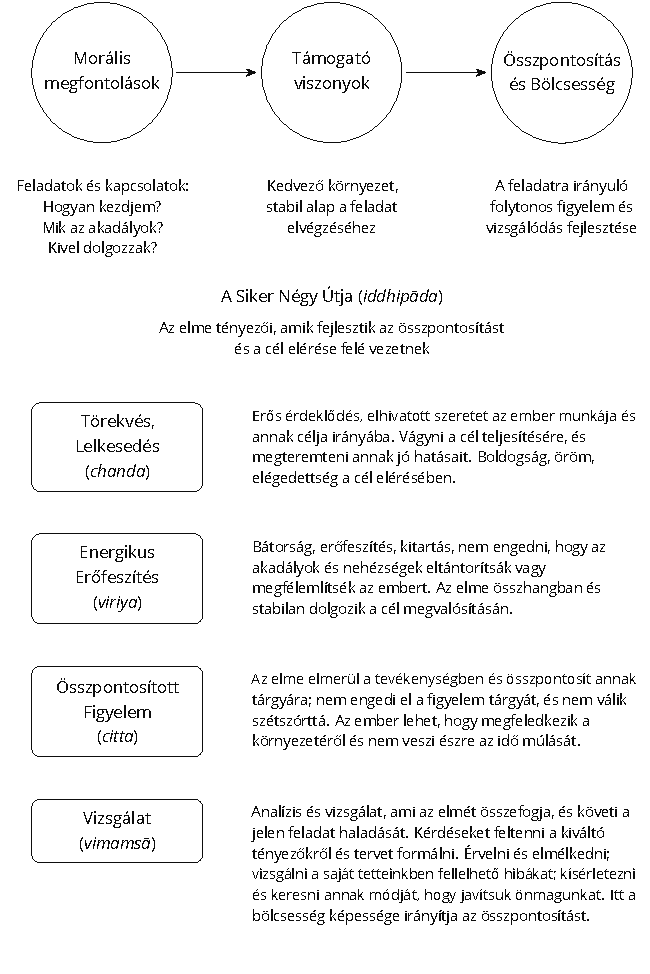
\includegraphics[width=0.95\linewidth]{./manuscript/tex/diagrams/paths-to-success-hu.pdf}
\end{figure}

\clearpage
\normalpagelayout

A csendes és nyugodt időszakok áldásnak számítanak. Mindig is értékeltem
egy stabil rutint, ami hosszú időszakokat enged a koncentrált munkára
vagy intenzív gyakorlásra. Más részről, akadályok és konfliktusok is
garantáltan jönni fognak.

Nem kell amiatt aggódnunk, hogy a meditáció meg fogja oldani minden
problémánkat, és nem lesz mit tennünk. A meditáció nem
probléma-megoldás. Ez az éberség olyan gyakorlása, ami túljut a belső
akadályokon és szembe néz a külső problémákkal, ahogy azok elénk
kerülnek. Ha egy fontos ügyet kell elintéznünk, segít, ha előbb
kitisztítjuk a fejünket. Viszont pusztán az, hogy ülünk a párnán mintha
túlhaladtunk volna minden problémán, a jelenre való tudatlanságot
gyakoroljuk, nem a tudatosságot.

Szándékosan szembe nézni és jó képességgel megbirkózni ezekkel arany
esélyt ad arra, hogy az elme képzését a korábbi korlátokon túl
fejlesszük. A zavaros káosz gazdag a lehetőségekben, hogy gyakorlati
úton fejlődjünk és tanuljunk.

Nem magukat az érzéseket keressük, nem különleges érzéseket próbálunk
létrehozni a meditációval, nem azt a helyzetet keressük, ahol mindig
minden jól megy nekünk. A kellemes, kellemetlen, semleges érzések
önmagukban nem adnak nekünk helyes megértést, ha követjük a befolyásukat
és gépiesen reagálunk rájuk. Az éberségnek észre kell vennie az
állandótlanságukat és bizonytalanságukat. Akkor megértéssel látjuk mi a
jótékony, és mi a kártékony a jelen helyzetben.

\keywords{csónak a folyón, én és enyém}

Könnyű a meditációt gyakorolni, vagy nehéz? Egy hasznos kép amire
gondolhatunk, ahogy egy csónak halad a folyón. Amikor a csónak áruval
töltött ládákkal van megrakva, a sok teher alatt nehezen és lassan
halad. Épp, hogy a víz felett tudja tartani magát.

Azt szeretnénk, hogy a csónakunk gyorsan haladjon, nem igaz? De
ugyanakkor ragaszkodunk mindenhez amivel megraktuk. Könnyítenünk kell a
csónakon, elengedni az `én' nehéz súlyát. Mi hozzuk létre az `én' és
`enyém' terhét. Mi hozzuk létre a benyomást, hogy `ilyen voltam, ilyen
vagyok, ilyen kell legyek'. `Az az enyém volt, ez az enyém, ez meg
akarom tartani, azt meg kell szereznem'. Ez a súly húzza le a csónakot.

Az érzés, hogy elég, ami van, megteremti a teret a nagylelkűségre. Az
elégedettség a gyakorlás folyamatos része, nem egy rögzült, feltételhez
kötött állapot. A tettek és a tanulás mint egy patak folynak az
elégedettségből. Mikor azt gondolom, `kész leszek elkezdeni, mikor már
megvan a \ldots{}', az elégedetlenség köti le a gondolataimat és folyton
megszakítja a koncentrációmat a jelen helyzetre.

\keywords{jótékony gondolatok, béke}

Viszont amikor azt gondolom, `nem vagyok jó ebben, de ennyi is elég,
hogy elkezdjem', elfogadni a jelen határaimat energiát ad a cselekvésre.
Végül gyakran többet is tudok tenni mint képzeltem.

A gondolkodás rossz hírnevet kap a meditációs könyvekben, de a tiszta
gondolatok megalapozzák a feltételeket a helyes hozzáállás fejlődéséhez.
Az elharapózó, kényszeres gondolkodás valóban fájdalmas tapasztalat, de
ha meg akarunk állítani minden gondolatot, mellé lövünk a célnak.

Vedd észre, hogy a jótékony gondolatokat megelégedettség és béke követi.
Erkölcsös tetteinket tudatosan felidézve kialakul a stabilitás és
ön-tisztelet érzete. Bízunk magunkban, hogy elengedjük ami fölösleges,
mert érezzük, hogy ami van az már elég.

Ha fejben akarjuk megoldani, a gyakorlás gyorsan bonyolulttá válik. A
meditációban, a testen keresztüli éberség egy megbízható irány: Az
érzéseket és elme állapotokat figyeljük, ahogy jönnek és mennek,
nézőpontunkat áthelyezzük, és nem magunkkal vagyunk elfoglalva. A
bonyolult kérdéseket magunk mögött tudjuk hagyni, mert már nincs
szükségünk a válaszokra.

\keywords{könnyű csónak, élvezetes tanulás}

Mi teszi lehetővé, hogy tovább tanuljunk és fejlődjünk? Az utazás akkor
a legélvezetesebb, amikor a horizont egyre tovább tágul, a korábbi
korlátainkon túl. A horizontot nem azzal tágítjuk, hogy messzire
utazunk, hanem azzal, hogy új szemmel látunk. A vágy, hogy megtartsuk
azt, amiről azt gondoljuk mi vagyunk, határozza meg a jelen korlátunkat.

A csónak könnyű, amikor üres az éntől és enyémtől. Nagy távolságokat
tesz meg dráma és zaj nélkül. Mi történik, ha a csónakban ülünk, és
valaki a csónakjával nekünk ütközik? Rákiáltunk, ellökjük az evezővel,
és egész nap erről panaszkodunk. Ez mind lehet, hogy jogos, de tönkre
tettük a napunkat a saját rossz társaságunkkal. Nehéz ebben a
bölcsességet látni. Mi történik, ha egy üres csónak ütközik nekünk?
Honnan eredt a korábbi harag és negatív indulat?

Hajlamosak vagyunk az én és enyémről szóló történeteket gyártani, akár
valós, akár képzeletbeli események alapján. Ha komolyan vesszük ezeket,
és valóságot adunk nekik, a történetek kezdenek irányítani minket, és
korábban nem létező problémákat hozunk létre.

\enlargethispage*{\baselineskip}

Előfordul, hogy ülünk a meditációs párnán, és vitákat kezdünk eljátszani
a képzelet bábjaival. Komoly az ügy, nekünk kell nyerni! Módszeresen
végig gondolni egy problémát hasznos eszköz, de önmagunk felé irányuló
szimpátiára és kedvességre is szükség van az építő jellegű belső
bárbeszédhez. Másként, amikor az én magával beszél, rossz társaságban
találja magát.

\keywords{aki tud önmagán nevetni}

Meglepő, mennyire fel tudjuk húzni magunkat egy olyan helyzettel
kapcsolatban, ami még meg sem történt. Segít, ha tartunk egy csipet
humort az oldal zsebünkben, vészes komolyság esetére. A görög filozófus,
Epiktétosz mondását felidézve, `Aki tud önmagán nevetni, sosem fogy ki a
nevetni valóból.'

\keywords{az érzékek egyszerűsége, elengedés}

A meditáció gyakorlásában visszaálltjuk a helyes szemléletet azzal, hogy
visszatérünk az érzékek egyszerűségéhez. A történeteket, ha vannak, a
változó körülmények nézőpontjából szemléljük. Az érzékek vizsgálatával
egy alapvetőbb valóságra alapozzuk a figyelmünket. A kellemes érzet
ilyen, ahogy most tapasztaljuk, a kellemetlen érzet ilyen, a semleges
érzet ilyen, kezdete van és vége, változik és üres.

A gyakorlásban nem az lesz értékes, hogy sietve eredményeket halmozunk
fel, hanem, hogy teret hagyunk az elengedésnek és türelemnek. Van amikor
cselekedni kell, de meglepően sokféle nehézséget megold az egyszerű
türelem. A sértettség vagy sürgető fontosság érzése magunkból ered. A
visszafogottság biztonságos nézőpontot nyújt ilyenkor, magunkkal és
másokkal szemben is. Engedjük a csónakunkat csendben tovább úszni.

%\chapter{Csontok}

\keywords{testi fájdalom meditáció közben}

\noindent Még ha jó testtartással is ülünk, előbb vagy utóbb valami
valahol fájni fog. A jó testtartás minimalizálja a szükségtelen
kényelmetlenséget, de nem tudja teljesen megszüntetni. A fájdalom és
kényelmetlenség ténye együtt jár azzal, hogy van testünk, de nem azért
meditálunk, hogy kínozzuk magunkat, és ügyelhetünk arra, hogy elkerüljük
a sérülést.

A testi fájdalmat vizsgálhatjuk azt mint a meditáció tárgyát,
figyelhetünk a test egy másik területére, ahol nincs fájdalom, vagy
változtathatunk a testtartásunkon.

Ha a megszokott reakciónk a fájdalomra szorongás, ellenszenv és
nyugtalanság, akkor a vizsgálódás hasznosnak bizonyulhat. Emlékezz, hogy
a szándékod az, hogy jót akarsz magadnak. Ezután vizsgáld, figyeld meg a
fájdalmat, hogyan mozog a testben, hogyan keletkezik és múlik el
hullámokban. `Ki az, aki szenved? Változik ez? Hol van a tudatosság, ami
ezt tudja?' Ez megváltoztatja miként észleljük a fájdalmat. A
tapasztalatunk megváltozik, egy vészhelyzetből amit azonnal meg kell
oldanunk, egy jelzéssé, amit választásunk szerint félre tehetünk egy
időre.

Lehet, hogy a fájdalom nem jelent sérülést, mint például az ahhoz
hasonlítható kényelmetlenség, amit akkor érzünk, mikor végig kell ülnünk
egy hosszú utat a buszon. Választhatunk, hogy a figyelmünket a test egy
másik részén tartsuk. Vagy, a figyelmet módszeresen végig vezethetjük a
test különböző részein, megfigyelve a helyet, ahol nincs fájdalom, és
meditációnkat így folytatjuk, annak a területnek az érzeteit szemlélve.

Egy érdekes gyakorlat pontosan meghatározni, hol húzódnak a fájdalmas
terület határai. Éles ez a határ, vagy határozatlan? Rögzítve marad,
vagy fokozatosan más irányba tolódik? Az ilyen vizsgálat közben
megismerjük a fájdalom keletkező és elmúló természetét. Ezután már nem
olyan nagy ügy. Nem kell ellenszenvvel reagálnunk rá, tudunk hagyni némi
szabad teret a kellemetlen érzeteknek, hogy hadd legyenek.

Amikor eldöntöd, hogy ideje megmozdulni, mielőtt mozdulnál, állj meg egy
pillanatra és határozd meg tisztán a szándékot: `A testem iránti
együttérzésből mozdulok. Megváltoztatom a testtartásom, mert azt
kívánom, hogy a testem jól érezze magát és egészséges legyen.' Ezután
helyezd át a lábaidat, vagy válts testtartást. Ez egyben tartja az
éberség folytonosságát, és így nem az ellenszenvre vagy nyugtalanságra
reagálunk.

\keywords{a test vizsgálata, csontok, az 'én' képe}

Az ülő meditáció után, átválthatunk álló helyzetbe és hagyjuk az
ízületeket és izmokat ellazulni. Az álló helyzet több figyelmet igényel
az egyensúly megtartására, így a csontok, a test tartóelemei, jobban
érezhetőek.

A csontok a test központi, merev részeit képezik, amik meghatározzák az
alakját, mit képes és képtelen tenni. Csontok nélkül, a testünk egy
formátlan húspaca lenne. Csontokkal belső struktúrát nyer, ami megadja a
külső megjelenését, amit jól ismerünk. A tükörbe nézünk és azt
gondoljuk, `az én vagyok'.

\clearpage
\thispagestyle{empty}\mbox{}
\photoFullBleedPlaceholder{%
  TODO: Illustration of standing meditation.%
  \illustration{Álló Meditáció Testtartás}%
  \label{illus-standing-meditation}%
}
\clearpage

Mennyire vizsgáltuk meg a képet, mielőtt magunkat láttuk benne? Egy
rövid körvonal, kontraszt és szín máris kiváltja az `én' kép
megjelenését. Viszonylag állandó képünk van magunkról, a jelenben a több
évvel ezelőtti önmagunk képével azonosulunk. Mivel a változás lassú,
egyre kevesebb és kevesebb kulcs jellemzőre hagyatkozunk, hogy
felismerjük a tükörben látható képet.

Ha közelebb hajolunk és több jellemzőt látunk, vagy magunkat egy
szokatlan szögből mutatja egy fotó, percekbe is beletelhet mire el
tudjuk dönteni, kit látunk. Mi határozza meg ez a képet? Ha a csontok
egy kissé mások lennének, a testnek más alakja lenne, és ez
megváltoztatná nem csak a külsőnket, de azt is, hogyan élünk.

\keywords{álló meditáció módszere, álló testtartás}

Állj egyenes, de rugalmas helyzetben, fordíts egy kis idő arra, hogy
megtaláld a kiegyensúlyozott tartást. Helyezd a lábfejeket
vállszélességbe, a térdeket engedd ellazulni és kissé behajlani, hogy
aktív részük legyen a test megtartásában. Ne zárd az ízületeket
egyenesre, az megfeszíti őket és a tartásod merevvé válik. Tartsd a
lábfejeket párhuzamosan, a lábujjakkal egyenesen előre mutatva. Forgasd
a csípőt előre a vízszintes vonal mentén, kissé behúzva az alsó részt. A
mozdulat ahhoz hasonlít, mintha egy vödröt fordítanál a felső nyílással
magad felé.

Döntsd a tested jobbra-balra kissé, és érezd ki a súlypontot. Fejleszd
azt az érzést, hogy te tartod a tested egyenesben, hogy ne dőljön el. A
test egyensúlyát jobb a sarkok felett tartani, mint előre dőlni és a
lábfejekre nehezkedni.

Tartsd a vállakat elég szélesen ahhoz, hogy megnyissák a mellkast a
könnyű légzéshez, de nem olyan szélesen, hogy feszültté váljanak. A
kézfejeket kényelmes például a combokon tartani, körülbelül a pont
fölött, ahol a zsebek vannak egy nadrágon.

Engedj magadnak rugalmasságot, végezz kis változtatásokat a tartáson,
ahogy az izmok hozzászoknak a helyzethez. Érezd ki az állásban az
egyensúlyt és figyeld a testet ahogy így tartod. A gravitáció lefelé
húzza, nyomást hoz létre a földön. Ha úgy jobb, behajthatod a kezeket a
has előtt, egyik tenyér a másikon, kényelmes helyzetben.

A szemek lehetnek nyitva vagy csukva. Ha álmos vagy jobb, ha nyitott
szemmel meditálsz, de tartsd a tekinteted a magad előtti pár méteren. Ha
egyenesen előre nézel, a figyelem iránya kifelé fordul, és az ablakokban
látható mozgás elvonja a figyelmed.

Ha becsukod a szemed, de erőltetettnek és fájdalmasnak érzed, figyeld
hova irányul a szem fókusza, amikor becsukod. Ha befelé húzódik, mintha
egy közeli tárgyra fókuszálna a szemhéjak mögött, a szemgolyó belső
oldalán lévő izmok erőlködnek, hogy befelé húzzák azokat, ez a
feszültség szárazságot és könnycsordulást is okozhat.

A hagyományos Buddha szobrokon a Buddha szeme kissé nyitva van. Ő éber,
nem alszik. Ne zárd a szemhéjakat szorosra, gyakorold ellazítani azokat;
engedd le őket nyomás nélkül. Bár a szemhéjak majdnem zárva vannak,
képzeld azt, hogy egy távoli dologra nézel, ez hagyja ellazulni az
izmokat. Egy keskeny sáv nyitva marad, némi fényt enged be. Az is segít,
ha megmasszírozod a belső oldali szemizmokat, a nagyujjak hegyével
körkörös mozgásban.

Vegyél egy lélegzetet, és figyeld, hogyan változik a testtartás légzés
közben. A rekeszizom behúzza a levegőt, a has előre mozdul, hogy helyet
adjon. A kulcscsontok megemelkednek, a mellkasi bordák kifelé nyílnak, a
test súlypontja kissé elmozdul.

Van valami, ami korlátozza a légzést? Ellenőrizd, hogy egyenesen állj, a
váll ne görnyedjen előre, ami gátolja a nyitott légzést.

Figyelj a fej egyensúlyára, találd meg a pozíciót, ahol a fej a saját
súlyával egyensúlyban ül a gerinc tetején, nem dől előre vagy húzódik
hátra. Irányítsd a tekintetet kissé lefelé, ahelyett, hogy egyenesen
előre néznél, mert a jövés-menés elvonja a figyelmed. Húzd be az állat
könnyedén, ne engedd előre kitolódni, irányítsd a tekintetek pár
méterrel magad elé a földre. Engedd a fejtetőt kicsit megemelkedni,
mintha tartaná az eget.

A fej pozíciója nagy mértékben befolyásolja a felsőtest tartását. Mivel
sokat ülünk székeken, kialakul a szokásunk, hogy a fejet előre tolva
tartjuk, ez megfeszíti az hátizmokat a gerinc mentén. Ezeket az izmokat
nem tudjuk tudatosan irányítani, de kipróbálhatod, milyen érzés kissé
visszahúzni a fejet. Érzed ki az egyensúlyt, ahol a hátizmok ellazulnak.

Kiegyensúlyozott testtartásban a csontok úgy ülnek egymáson, mint az
óvatosan egymásra helyezett kövek. Ha a gerinc jó tartásban van, a
gravitáció elég, hogy stabilan tartsa. Ez kellemes, könnyed egyensúlyt
teremt erőltetés nélkül.

\enlargethispage*{\baselineskip}

\keywords{testhez való hozzáállás, analitikus elme, jószándék}

Ha túl analitikus hozzáállással közelítjük meg a test vizsgálatát, ez
groteszk és sokkoló benyomásokat kavarhat fel. A magunk felé irányuló
jószándék tartja a meditációt egyensúlyban, és hozzáállásunk jótékony
marad.

Az intellektus működése során elvont fogalmakat épít, figyelmének
tárgyait elkülöníti az egésztől. Mikor a testet szemléli, lehet, hogy
annak különböző részeit absztrakt és élettelen tárgyként tekinti.
Emlékezzünk, hogy nem azért gyakoroljuk a meditációt, hogy a testtel
szemben ellenszenvet vagy elidegenedést keltsünk. A meditáció tiszta
megértése akkor működik jól, amikor a dolgokat a környezetükkel együtt
látja, semmi nem létezik elszigetelve, üres térben. A tudatosság
befogad, nem kizár, és ehhez a hozzáállásunk része kell legyen a nyitott
elfogadás és jószándék.

Ez a hozzáállásbeli különbség egy történetre emlékeztet Platónról és
Diogenészről. Platón éppen egy előadást tartott a diákjainak Athénban az
Akadémián, és az `ember' fogalmát úgy határozta meg, mint `tollatlan
kétlábúak'. Úgy esett, hogy Diogenész hallotta ezt, és mivel kedvelte az
gyakorlatias vicceket, behozott az Akadémiára egy kopasztott csirkét, és
feltartotta Platónnak, ``Íme! Hoztam neked egy embert.'' Úgy
gondolhatta, ez bemutatja, hogy bizonyos környezeti jellemzők hiányoznak
az ember túlságosan intellektuális meghatározásából, mint `tollatlan
kétlábú'.

A csoport az Akadémián kiegészítette a meghatározást, ``\ldots{} lapos
és széles körmökkel'', ami kielégítette az intellektuális tárgyalásukat,
de alighanem nem értették meg mire mutatott rá Diogenész.

\keywords{az egész testet megtapasztalni}

Figyeljük a testi érzéseket a belégzés és kilégzés közben. Irányítsd a
figyelmet befelé, éberen a benyomásra, hogy `a test ilyen'. Az elme nem
keres, nem a világban jár valahol. Nem igényel semmit, ami itt van az
elég. Éberséggel látjuk a testet, a lábfejeket, a lábakat, a hasat, a
mellkast, a karokat, a vállakat, a nyakat és a fejet. Az test egy
egészet alkot, egy mozgó benyomás, érzékeny a lélegzetre.

A testet így figyelni olyan, mint az esőt nézni. Nincs tennivaló, semmit
nem kell eldönteni. Az eső tovább folytatja a dolgát anélkül, hogy be
kellene avatkoznunk.

\keywords{tiszta megértés, testre irányuló tudatosság, kioltani a haragot és vágyat}

A kártékony gondolatokat hasonlíthatjuk a szélben kavargó porhoz:
elhomályosítja a képet, nem látunk tőle semmit. A Buddha az éberség
hatását az elmére az esőhöz hasonlította, ahogy kimossa a port és
megtisztítja a levegőt. `Szüntesd meg az ilyen (kártékony) gondolatokat
és kérdéseket, ahogy az eső elmossa a port; A szívben elcsitulnak a
gondolatok, és helyben eléri a béke állapotát.'\footnote{\href{https://suttacentral.net/iti87/en/sujato}{Iti
  87}, A Látás Pusztítói}

Az elmére való éberség megállítja a kártékony jellemzők keletkezését,
fejleszti a jótékony jellemzőket, és így megtisztítja az elmét.
Észrevehetjük, hogy a világot nem egy rögzített módon tapasztaljuk: nem
elzárt, külső szemlélők vagyunk, mintha egy magunktól különálló világra
néznénk az ablakon át. Aktív szerepünk van a világ létrehozásában, amit
tapasztalunk, hiszen mi alkotjuk a benyomásait a figyelmünk módján
keresztül.

Amikor megalapoztad a tiszta megértést, és észreveszed, hogy az elme
egyre tisztább és stabilabb, vedd szemügyre, mi tette lehetővé ezt a
változást? Mit tettél? Mit \emph{nem} tettél? Nem kellett az érzéki
benyomásokat manipulálnod, vagy küzdened a gondolatokkal és érzelmekkel,
elegendő volt megváltoztatni a figyelem módját.

A figyelmünk módja hozza létre a referencia keretet, amiben
megtapasztaljuk az érzékek világát az észlelések és emlékek felfogásától
függően. Ez egy folyamat, ami egy bizonyos hozzáállást produkál, mint
egy, az időt feldolgozó függvényt, aminek eredményétől függően
felismerjük és értelmezzük önmagunkat a jelenben.

A figyelem változását arra használjuk, hogy ne tápláljuk tovább a
kártékony mentális tényezőket. A közvetlen tapasztalat szemszögéből,
annak megfelelően ahogy a dolgok vannak, végük szakad, a folytatáshoz
szükséges referencia pont nélkül.

Röviden úgy mondjuk, az elmére való éberség megtisztítja az elmét.

A testi tudatosság felé fordulunk, ami kioltja mind a haragot és vágyat.
Megváltoztatja a figyelmünk keretét, hasra esnek mintha kihúztuk volna
alóluk a szőnyeget. A zsúfolt, kritikus és haragos gondolatok olyanok,
mint egy zajos műsor, vagy a hírek a tavalyi újságban. A témája már nem
érdekel minket, elvesztette a fontosságát, folyton csak körbe-körbe jár.
Tedd le a gondolkodást, mint egy fáradt túrázó a nehéz hátizsákot, és
maradj a test éber figyelmével.

Időnként elvonja valami a figyelmünket, vagy elkezdünk álmodozni; mindig
térj vissza a légzéshez és az álló helyzet testi érzéseihez. Ha állás
közben csak történetekről és belső fantáziákról gondolkodunk amíg meg
nem szólal a harang, azzal nem a belátás meditációt gyakoroljuk\ldots{}
hanem a buszra várakozást.

\clearpage

\keywords{emlékek mint én, történetek az énről}

Vizsgáld az elme állapotát mint tapasztalatot. A test észlelése és az
érzései azelőtt jelennek meg, hogy az `én' észlelését felépítenénk
belőle. Mire emlékszünk önmagunkról? Ha elfelejtjük, amikor tegnap
valaki gorombán ránk kiabált, vagy emlékezünk, amikor barátainkkal
töltöttük az időt, ez megváltoztatja miként tekintünk önmagunkra?

Ez a kapcsolat az emlékeink, érzéseink és elme állapotunk között folyton
változik. A felfogott képek folyton változnak, az éber tudatosság
megismerésével a bizalmat abba helyezzük, ami ismeri ezt a változást.
Ezzel a változást egy nagyobb képen belül láthatjuk, és nem ragadunk meg
a félelemben. Önmagunk képét egy aktív folyamat hozza létre, részt
veszünk benne az emlékeinkkel, azok újra-értelmezésével. Felépítünk egy
történetet magunkról a múlt emlékeiből, és megválasztjuk mit teszünk
most.

\keywords{csontok, a test részei, megfelelni akarás, a külső megjelenés bírálata}

A testet és annak részeit szemlélve az elmét a változó benyomásokra
összpontosítjuk, mielőtt az `én' képe megjelenik. Ez a folyamat
lefegyverzi az ön-bírálatot, a félelmet és elvárásokat, amik mint a
mocsár lehúznak minket.

\enlargethispage*{\baselineskip}

Figyeld az érzést, ahogy a csontok kapcsolódnak egymáshoz az
ízületeknél. Megjelenik egy belső struktúra érzete, a struktúra ami a
testet belülről tartja. Merev darabok, egyik vég a másikhoz kapcsolódik,
egymásra rakva egyre magasabbra. A lábakban érezzük a merev csontokat,
ahogy tartják a testünket. Az érzés a gravitációról és nyomásról
árulkodik. A csípő csont a lábakon nyugszik, a felső test ehhez
kapcsolva mozog. A mellkas bordái szétnyílnak és összehúzódnak a
légzéssel. A gerinc ív alakban tartja a súlyt. A fej ott ül a gerinc
tetején. A koponya csontjai megfeszítik az arcbőrt.

A testünk darabokból áll. Darabokból, amik egyes helyeken merevek, más
helyeken puhák és rugalmasak. Ezek együttállása adja meg a formáját.
Amikor egy személyre nézünk, nem látunk mást, mint a hajat a fejen, a
szőrt a testen, körmöket, fogakat és bőrt. Ebből építjük a személyt --
elég a másodperc törtrészéig rápillantanunk, felismerni egy körvonalat
vagy jellemzőt, és azt gondoljuk, `Ez én vagyok. Jól nézek ki?'

Egyes helyzetekben láthatjuk a fokozatos felismerést az általánostól az
egyéniig, például amikor valakit látunk a ködben sétálni. Először
észrevesszük, hogy ez egy `személy' alakja, azután férfi vagy nő. Lehet,
hogy valaki akit ismerünk? Végül egy részlet kiváltja egy barátunk
felismerését és eszünkbe jut a neve. Mindez az észlelés képeinek
világában játszódik le.

Szokásunk, hogy a saját testünket, és másokét, egy töretlen egységként
látjuk, egyetlen dologként. Ebből a nézőpontból kialakul a megrögzött
gondolat, hogy van egy ideális formája és állapota. Elvárjuk, hogy a
testnek legyen bizonyos formája, magas vagy alacsony, és a további
jellemzői.

Ezek világi bírálatok, képek amit a kultúra amiben felnőttünk alakított
ki bennünk. Az egyik kultúra a vékony, a másik a telt testet tekinti
ideálisnak, és ezek a kulturális ideálok is változnak egyik generációról
a másikra. A hirdetések és a média üzenetei megerősítik ezeket az
elvárásokat és gondolat nélkül hiszünk bennük. Amikor közelebbről
szemügyre vesszük, azt látjuk, ezek egy ferde tükör képei, nem egyeznek
a valósággal.

\clearpage

\enlargethispage*{3\baselineskip}

\begin{figure}[h]
\caption{Experience and Illusion of Self}\label{fig-illusion-of-self}

\centering

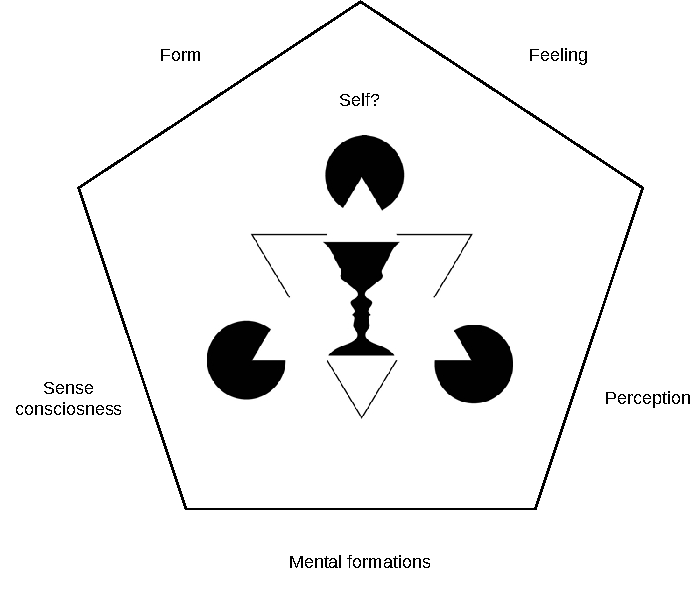
\includegraphics[width=80mm]{khandhas-self-illusion.pdf}

\bigskip

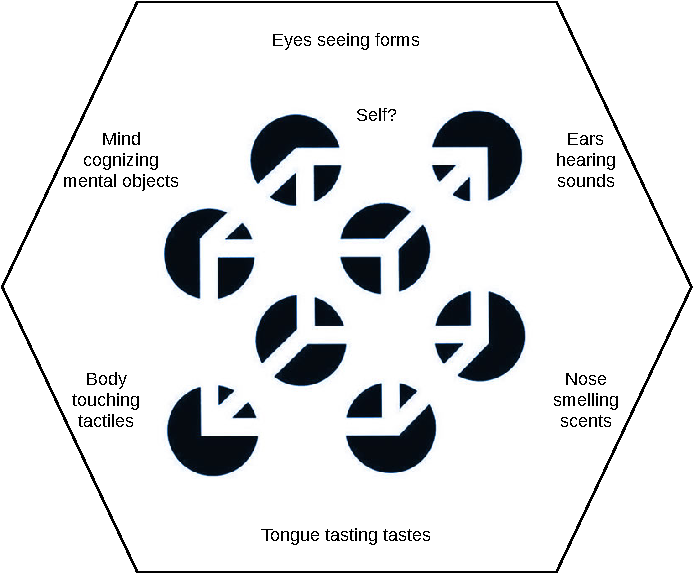
\includegraphics[width=80mm]{senses-self-illusion.pdf}

\bigskip

{\small
We experience a self, which has no substance beyond that experience.
Above, conditioned expectations create filled-in shapes which we \emph{experience}, but are not there.
The Kanizsa Triangle, Rubin's Vase and Subjective Necker Cube are examples of illusory contours.
}

% FIXME TODO translate figure text

\end{figure}

\clearpage

Lehet, hogy mi sokat gondolunk arra, hogy mások mit gondolnak rólunk, de
\emph{mi magunk} mennyit törődünk mások küllemével? Ha magamat figyelem,
nem foglalkozok sokat más emberek kinézetével. De én zavarban tudom
érezni magam, és azt képzelem \emph{ők} biztos \emph{rólam}
gondolkodnak. Mikor, valójában, annyit gondolnak rám mint én rájuk --
alig, ha egyáltalán. A saját életükkel vannak elfoglalva, mint ahogy én
is az enyémmel.

Az önbírálatunk nyomása mellett, elképzeljük mások hogyan bírálnak
minket. Mivel nem tudhatjuk és nem irányíthatjuk mit gondolnak, az elme
belső párbeszédével megpróbáljuk megteremteni ezt a tudást és
irányítást, ami illúzió marad. Amikor lejátsszuk ezeket a belső
párbeszédeket, élvezzük ezt a megfoghatatlan irányítást. Viszont
lemaradunk arról a szabadságról, ami az irányítás igényének
elengedéséből születik.

\keywords{a test részeinek éntelen jellege}

Megfigyelhetjük az aggodalom feltételektől függő természetét, amikor a
test egyes részei elválnak. Sokat foglalkoztathat minket a hajunk
például, de csak addig, amíg a fejünkön van. Amikor a fodrász levágja,
nem törődünk a padlón összegyűlt hajkupaccal. Hasonló módon, mikor a
körmünket vágjuk, mikor van az a pont, amikor már nem `én' és `enyém'?

Így vizsgáljuk a testet, mint ami darabokból áll össze, és látjuk, hogy
a test nem egy bontatlan egység. Darabokból és részekből áll, amiknek
megvan a maguk természete, és aszerint viselkednek, nem hallgatnak a mi
vagy mások véleményére. Csontok, bőr, haj, fogak és körmök: olyanok
amilyenek, a saját természetüknek megfelelően.

\clearpage

A testünk egy áldás. Nem azért gyakoroljuk a meditációt, hogy
ellenszenvet keltsünk felé. Az egészség egy áldás, támogat minket
mindenben, amit teszünk. A Buddha az egészséget a legnagyobb kincsnek
nevezte.

\keywords{történetek mint álmok, testre irányuló tudatosság, szürke és élettelen állapotok, hála érzet}

Figyeljük a légzést, a test részeit, a jelen tapasztalatunkat. Azt
találjuk, hogy nem hordozzák magukkal az `én' és `enyém' történeteit.
Mivel mi hozzuk létre ezeket a történeteket, meg is tudjuk állítani
őket, nem vagyunk hozzájuk láncolva. A jelenségek függő kapcsolatokon
keresztül létre jönnek, a kapcsolat felbomlásával megszűnnek. Ez minden
ami történik.

A testre irányuló tudatosság enged a kívánságok szorításán és rávezet
arra, hogy szerencsések vagyunk, hogy itt lehetünk. Ehhez a figyelemhez
mindig vissza tudunk térni, egy belégzés és kilégzés elég ahhoz, hogy
emlékezzünk a keletkezésre és elmúlására. A kétségek olyanná válnak,
mint a sztorik egy régi újságban. A múlt szálait nehéz követni és
fáradtságos kibogozni, mintha valaki más álmait kellene értelmeznünk.

Ami valós, az mindig itt van a jelen tapasztalatunkban. Nem az válik
fontossá, hogy mik vagy kik vagyunk a történetben, hanem az, hogy a
figyelmünket a jelennek tudjuk szentelni.

\enlargethispage*{\baselineskip}

A tiszta szándéknak fontos szerepe van. Amikor nincs tisztán
elhatározott szándékunk, egyszerűen csak sodródunk. Nem kifejezetten
zavar minket, hogy itt vagyunk, de az elme szürke és élettelen, egy
jövőbeli időre vár, és addig próbál elbújni és láthatatlanná válni. Az
eredmény, hogy valóban szürkévé és láthatatlanná válunk. Semmi rossz nem
történik, de nincs semmi fény és öröm abban, hogy itt vagyunk.

Nem állunk meg elég gyakran, hogy észrevegyük mikor boldogok és
nyugodtak vagyunk. Amikor az elme tiszta és csendes, természetes módon
hálás azért ami itt van, és az áldásokért amit életünkben kaptunk.

A hálát nem lehet akarattal erőltetni. A gyakorlásban nem létrehozunk
valamit, hanem tiszta szándékkal felismerjük azt ami itt van. Nem erő
vagy képesség kérdése, ezek időhöz és körülményhez kötöttek. Az
elhatározás, a befelé irányuló felismerő figyelem nem egy adott
körülményhez kötött. Az eredmény a helyes szemlélet, amiben látjuk a
dolgok megfelelő helyét, és mit kell azokkal tenni -- vagy csak
megállni, figyelni és lélegezni.

%\hypertarget{uxf3ceuxe1n-1}{%
\chapter{Óceán}\label{uxf3ceuxe1n-1}}


\chapter{Csontok}

\chapter{Óceán}

\chapter{Cél}

\chapter{Csend}

\backmatter

%\input{./manuscript/tex/references.tex}

%\cleartorecto
\thispagestyle{plain}

{\fontsize{10}{14}\selectfont%
\setlength{\parindent}{0pt}%
\raggedright\label{copyright-details}%
\setlength{\parskip}{7pt}%

{\centering

{\LARGE\ccbyncnd}

This work is licensed under a Creative Commons\\
Attribution-NonCommercial-NoDerivatives 4.0 International~License.\footnote{%
\href{https://creativecommons.org/licenses/by-nc-nd/4.0/}{https://creativecommons.org/licenses/by-nc-nd/4.0/}}

}

You are free to:

\begin{packeditemize}
\item Share — copy and redistribute the material in any medium or format
\end{packeditemize}

The licensor cannot revoke these freedoms as long as you follow the license terms.

Under the following terms:

\begin{packeditemize}
\item Attribution — You must give appropriate credit, provide a link to the license, and indicate if changes were made. You may do so in any reasonable manner, but not in any way that suggests the licensor endorses you or your use.
\item NonCommercial — You may not use the material for commercial purposes.
\item NoDerivatives — If you remix, transform, or build upon the material, you may not distribute the modified material.
\end{packeditemize}

No additional restrictions — You may not apply legal terms or technological measures that legally restrict others from doing anything the license permits.

Notices:

You do not have to comply with the license for elements of the material in the public domain or where your use is permitted by an applicable exception or limitation.

No warranties are given. The license may not give you all of the permissions necessary for your intended use. For example, other rights such as publicity, privacy, or moral rights may limit how you use the material.

% TODO confirm this notice with The Publisher

\thePublisher\ asserts its moral right to be identified as the author of this book.

\thePublisher\ requests that you attribute ownership of the work to \thePublisher\ on copying, distribution, display or performance of the work.

}


\emptyUntilEven

\end{document}
